%!xelatex = 'xelatex --halt-on-error %O %S'

\documentclass{thuemp}
\usepackage{url}
\usepackage{lipsum}  % 生产假书乱文的包,实际使用时可去掉
\usepackage{hyperref}
\begin{document}

% 标题,作者
\emptitle{基于JMAG软件的永磁同步电机仿真分析}
\empauthor{秦华谦}{魏亮亮老师}

% 奇数页页眉 % 请在这里写出第一作者以及论文题目
\fancyhead[CO]{{\footnotesize 秦华谦: 基于JMAG软件的永磁同步电机仿真分析}}


%%%%%%%%%%%%%%%%%%%%%%%%%%%%%%%%%%%%%%%%%%%%%%%%%%%%%%%%%%%%%%%%
% 关键词 摘要 首页脚注
%%%%%%%%关键词
\Keyword{JMAG,三相永磁同步电机}
\twocolumn[
\begin{@twocolumnfalse}
\maketitle

%%%%%%%%摘要
\begin{empAbstract}
  本次实验通过对 JMAG 的学习与应用,搭建了双层整距绕组4极表贴式三相永磁同步电机。在对电机本体运
  行机理和电磁特性分析的相关实验设计中,对比了绕组结构、极对数等对空载反电势、反电势谐波、转矩和转矩脉动
  等性能的影响。
\end{empAbstract}

%%%%%%%%英文标题、作者、摘要、关键词
\emptitleEn{Simulation analysis of three-phase permanent magnet synchronous motor based on JMAG}
\empauthorEn{Huaqian Chin}{Prof. Wei Liangliang}
\KeywordEn{JMAG, Three-phase permanent magnet synchronous motor}

\begin{empAbstractEn}
In this experiment, through the study and application of JMAG, a double-layer full-pitch winding 4-pole surface-mounted three-phase permanent magnet synchronous motor was built. In the related experimental design of the analysis of the operating mechanism and electromagnetic characteristics of the motor body, the effects of winding structure, number of pole pairs, etc. on the performance of no-load back electromotive force, back electromotive force harmonics, torque and torque ripple were compared.
\end{empAbstractEn}

%%%%%%%%首页角注,依次为实验时间、报告时间、学号、email
\empfirstfoot{2023-11-20}{2023-11-25}{21312683}{qinhq5@mail2.sysu.edu.cn}
\end{@twocolumnfalse}
]
%%%%%%%%!首页角注可能与正文重叠,请通过调整正文中第一页的\enlargethispage{-3.3cm}位置手动校准正文底部位置:
%%%%%%%%%%%%%%%%%%%%%%%%%%%%%%%%%%%%%%%%%%%%%%%%%%%%%%%%%%%%%%%%
%  正文由此开始
\wuhao 
%  分栏开始

%=================================================================
\section{概~~述}
\enlargethispage{-3.3cm}
\begin{figure}[H]
  \centering
  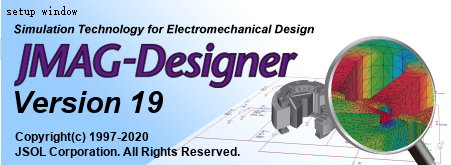
\includegraphics[width=0.8\linewidth]{./img/jmag.png}
\end{figure}
JMAG软件不同于其他用于电机仿真的Flux、MotorSolve、Ansys、Ansoft等,是一款针对电机
的电磁场的软件,它是日本的JSOL公司所研发,主要
用于各类电机电磁场的仿真分析。较其它类型的软件,
它具有奇特的工作界面, 种类繁多的材料属性库以及高
速且精准的计算分析等优势。

\begin{figure}[H]
  \centering
  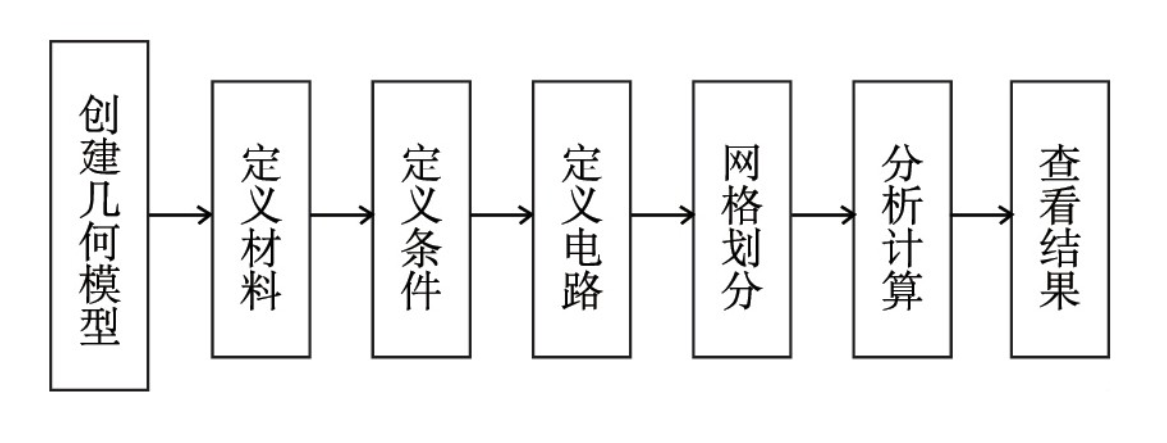
\includegraphics[width=1\linewidth]{./img/jmag_flow.png}
  \caption{Jmag建模流程}
  \end{figure}

电机的仿真模型在JMAG中可以通过多种方式来
建模,例如,可以通过在Geometry Editor中绘制,在
JMAG-Express中通过设置参数来建模,还可以通过
CAD导入的形式来完成建模。定义材料就是指将其物
理属性附加到所建模型中的相应部分。定义条件主要包
括三方面:

\begin{enumerate}
	\item 电机的运动方式
	\item 线圈的电流方向
	\item 边界条件
\end{enumerate}

定义电路就是指设定电机电路的连接方式和电路
的控制方向。网格划分是指对所建的模型进行划分,利
于有限元的计算。分析计算是指计算机对所建电机模型
计算的过程。查看结果就是查看分析电机的仿真参数。

接下来我将在JMAG软件中对一个表贴式三相永磁同步电机,并完成以下实验内容:

\begin{enumerate}
	\item 基本原理分析:搭建双层整距绕组4极表贴式三相永磁同步电机模型(y=3),进行仿真分析,分析电机的磁场分布、基本原理、空载性能和转矩、转矩脉动等。
	\item 绕组结构对比:搭建双层绕组4极表贴式三相永磁同步电机模型,基本模型参数如下,分别设计节距为y=1(集中),y=2(短距)和y=3(整距)的电机进行仿真,对比分析各电机的空载反电势、反电势谐波、转矩和转矩脉动(负载时,电枢电流峰值为10A)等性能。
	\item 极对数对比:搭建双层集中绕组表贴式三相永磁同步电机模型(y=1),基本模型参数如下,分别设计4极、8极和10极的电机模型进行仿真,对比分析各电机的空载反电势、反电势谐波、转矩和转矩脉动(负载时,电枢电流峰值为10A)等性能。
\end{enumerate}

%======================================================
\section{三相永磁同步电机}
\subsection{基本原理}
永磁同步电动机(PMSM),作为一种高效的电机类型,以其独特的构造和工作原理广受关注。
这种电机的特点是使用永磁体来提供所需的励磁力,这意味着它不需要电刷和励磁电流。
这些特性不仅降低了电机的维护需求,而且显著提高了电机的运行效率和功率密度。

1)结构: 永磁同步电动机一般由:定子,转子,端盖
等部件组成。

定子:定子是永磁同步电动机的主要部分之一,它由定子绕组和定子铁芯组成。
定子绕组围绕着铁芯进行环绕,这些绕组通过接收控制信号来调节输入电流的频率,
从而控制磁场的旋转频率,进而实现对电机转速的精确控制。

转子:转子是放置永磁体的部分,根据永磁体的放置方式不同,转子可以分为表贴式和内埋式两种。
在本次仿真中,使用的是表贴式永磁同步电机(SPM),其特点是永磁体直接贴在转子的外表面。

端盖:端盖作为电机的保护部分,起到封闭和支撑电机内部组件的作用,确保电机的稳定运行。

2)工作原理: 永磁同步电动机不能直接通三相交流的起动,因转
子惯量大,磁场旋转太快,静止的转子根本无法跟随磁
场启动旋转。

因此,永磁同步电机工作方式分为两种:一种
是通过变频调速器控制电机达到同步,一种是通过异步
起动方式来达到同步。

1)变频调速器方式:在这种方式下,电机的电源来自一个变频调速器。
在启动时,变频器逐渐提高输出频率,从零开始直至达到工作频率。
电机的转速随着变频器输出频率的增加而同步提高。
这种方式允许通过改变输出频率来精确控制电机的转速。

2)异步起动方式:永磁同步电动机的启动和运行是由
定子绕组、转子鼠笼绕组和永磁体这三者产生的磁场的
相互作用而形成。

在不需要调速的场合直接用三相交流电供电的方
法是在永磁转子上加装笼型绕组。

静止时,给定子绕组通入三相交流电,产生定子旋
转磁场;定子旋转磁场相当于转子旋转,在笼型绕组内
产生感应电流,形成转子旋转磁场。这两个磁场相互作
用,产生转矩,使转子由静止开始转动。

在刚开始转动的时候,转子旋转磁场的转速与定子
旋转磁场的转速不等,这样会产生交变转矩。

当转子旋转磁场几乎与定子旋转磁场同步时,转子
绕组不产生感应电流,转子上只有永磁体产生磁场,产
生驱动转矩!

所以,转子绕组来实现一个启动,启动完成后,转
子绕组不再起作用,由永磁体和定子绕组的磁场相互作
用,产生力矩。

高效率和高功率密度:由于其简洁的结构和强大的磁场,SPM电机通常拥有较高的效率和功率密度。
这使得它们非常适合需要轻量化解决方案的应用。

动力性能:SPM电机由于磁铁的直接作用,提供了优秀的动力性能,特别是在低速高扭矩的应用中表现出色。

磁场减弱操作的灵活性:当电流的相位移动并施加在d轴上时,即使是在SPM电机中,也会出现磁场减弱现象。
磁场减弱主要是通过在d轴上施加电流来实现的,这种电流足以削弱转子中的磁场。
结果是,尽管转速增加,但是转矩会减少。
SPM电机通过调整d轴电流,可以灵活控制转子磁场的强度,从而实现不同的运行状态,
适应各种不同的应用需求。这种控制策略对于需要在不同速度下运行的应用场景非常有用。

总体来说,SPM电机因其优越的结构特点和灵活的工作原理,在电动汽车、工业自动化等领域有着广泛的应用前景。

\subsection{总体架构}
三相表贴式永磁同步电机(Surface Permanent Magnet, SPM)是一种常见的永磁同步电机,
其特点在于永磁体直接贴在转子的外表面。这种设计使得电机在结构上更简单,
同时在某些应用场景中提供了更高的效率和更好的动力性能。

在SPM电机中,永磁体被安装在转子的外表面。
这种布局使得永磁体直接面对定子,从而最大化了磁场的效果。
转子的表面通常平整,以确保磁体的固定和保护。

永磁体的排列方式通常是有序且对称的,以保持磁场的均衡和稳定。
这种对称布局有助于减少振动和噪音,同时提高电机的整体效率。

磁场互动:在SPM电机中,当定子的旋转磁场垂直于转子上的永磁体(即q轴)时,
电机的运行类似于普通的永磁同步电机。这时,磁场直接与永磁体相互作用,产生驱动力。
% 插入模型图片
\begin{figure}[H]
  \centering
  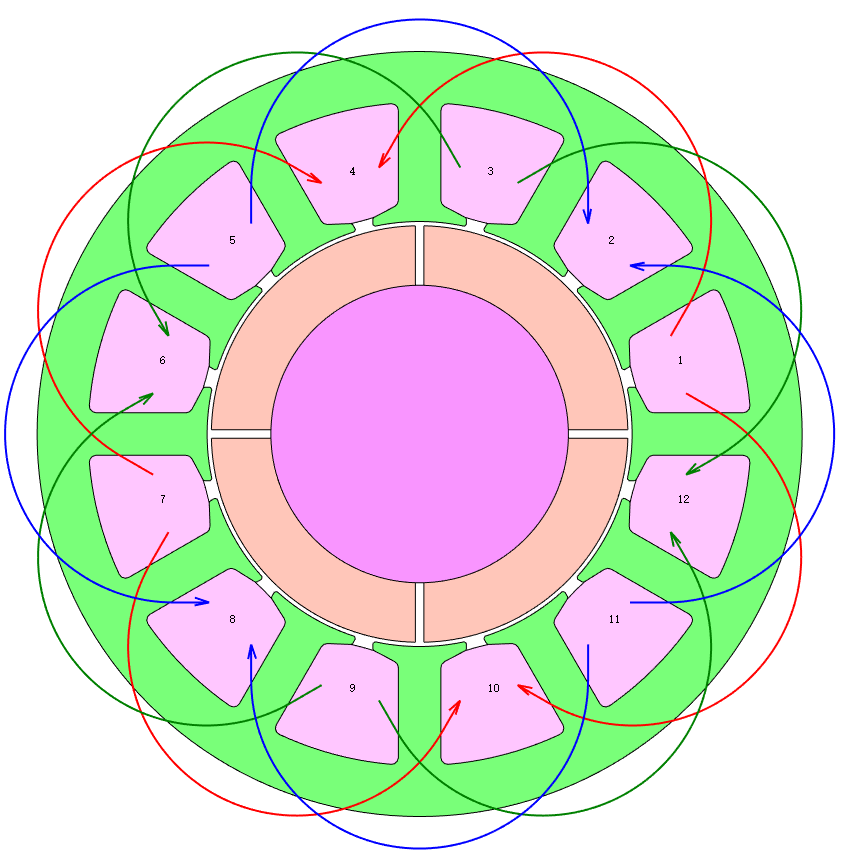
\includegraphics[width=1\linewidth]{./img/task1/model1.png}
  \caption{模型2D图}
\end{figure}

%============================================================
\section{Task 1:基本原理分析}

\subsection{基本模型与具体参数}
% 插入参数图片
模型设置如下图:
\begin{figure}[H]
  \centering
  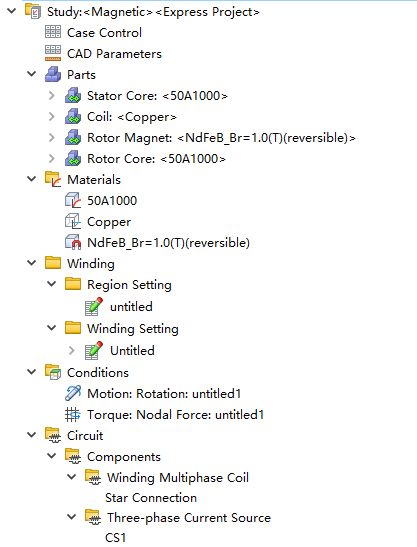
\includegraphics[width=1\linewidth]{./img/task1/model1-config1.png}
  \caption{模型管理器}
\end{figure}

具体参数:

\begin{figure}[H]
  \centering
  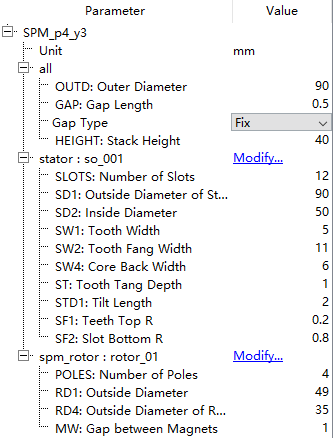
\includegraphics[width=1\linewidth]{./img/task1/model1-config2.png}
  \caption{尺寸参数}
\end{figure}

\begin{figure}[H]
  \centering
  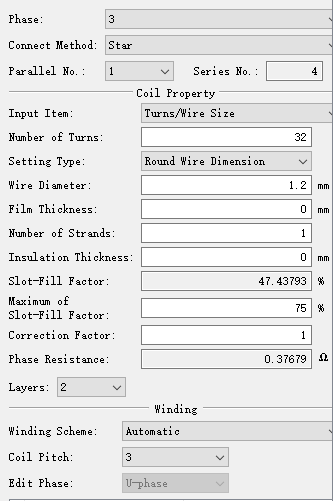
\includegraphics[width=0.8\linewidth]{./img/task1/model1-config-winding.png}
  \caption{绕组参数}
\end{figure}
% 插入负载、空载电路图
\begin{figure}[H]
  \centering
  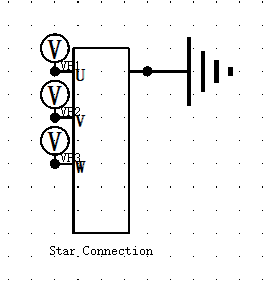
\includegraphics[width=0.8\linewidth]{./img/task1/noload.png}
  \caption{空载电路图}
\end{figure}

\subsection{磁场分布}

\begin{figure}[H]
  \centering
  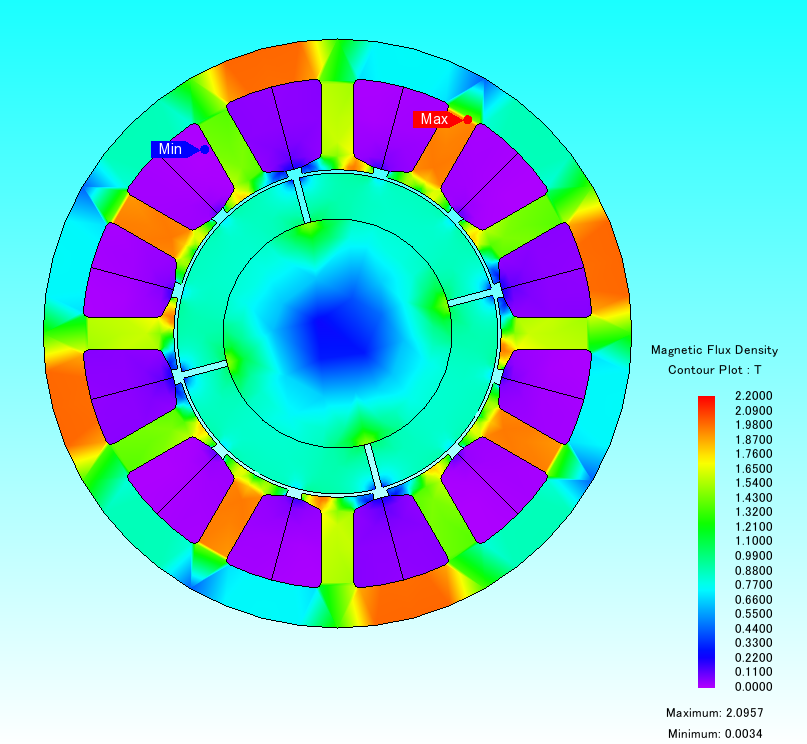
\includegraphics[width=1\linewidth]{./img/task1/mag-HotImg.png}
  \caption{磁场热力图}
\end{figure}

\begin{figure}[H]
  \centering
  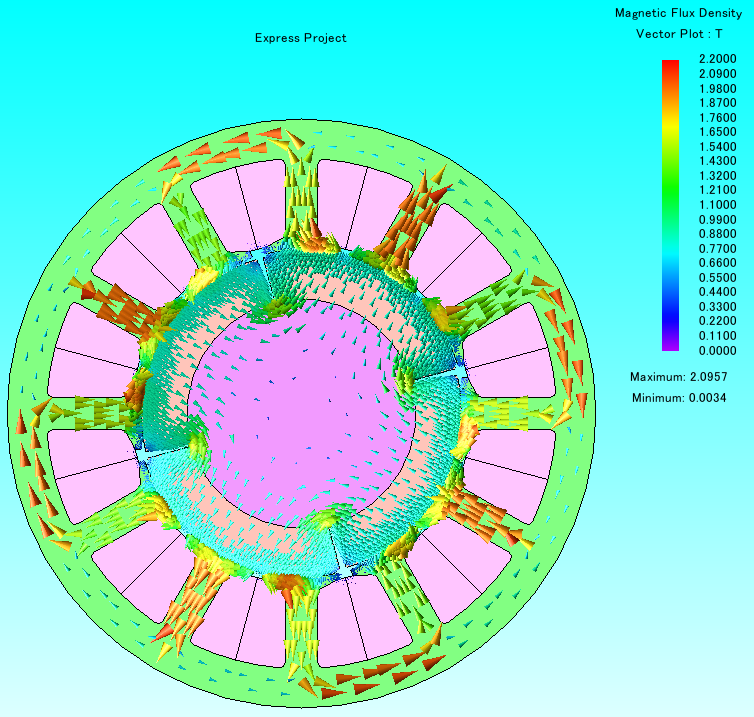
\includegraphics[width=1\linewidth]{./img/task1/mag-LineImg.png}
  \caption{磁力线分布图}
\end{figure}

\begin{figure}[H]
  \centering
  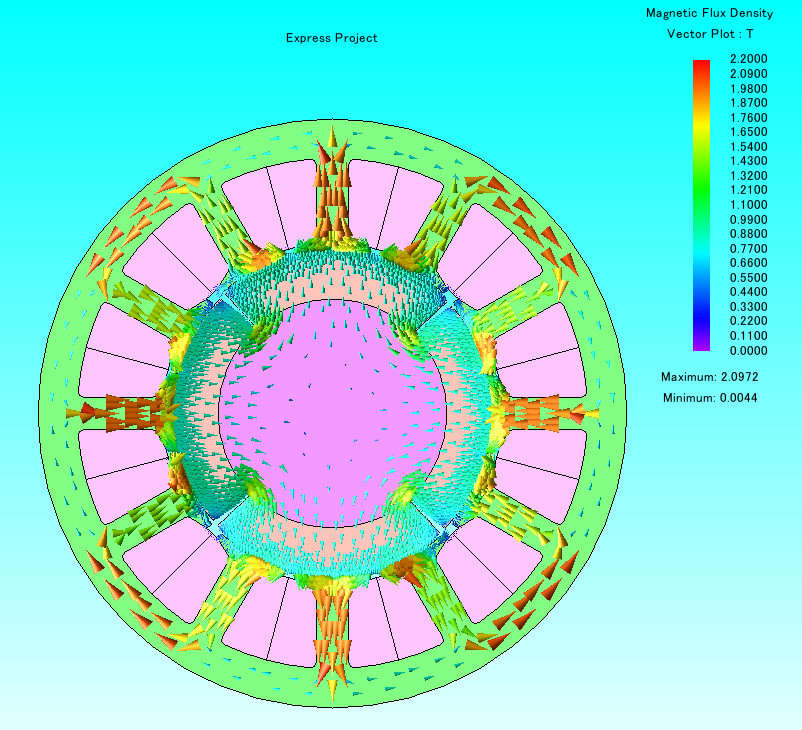
\includegraphics[width=1\linewidth]{./img/task1/mag-LineImg-turn45deg.png}
  \caption{磁力线分布图-旋转45deg后}
\end{figure}


\subsection{性能}
\subsubsection{电压电流波形推导}
永磁同步电机的转子磁动势为永磁
体产生: 永磁体磁动势$F_{pm}=H_c h_{pm}$式中,$H_C$表示永磁体的矫颁力,$h_{pm}$为永磁体的厚度
如图所示,永磁体的磁动势表示为波函数:

$$f_r=f\left(\gamma-\theta_r\right)$$

式中,$\gamma$表示空间位置,$θr$表示转子
位置角另外,提取永磁体磁动势的基波分量: $f_{r1}=F_{pm1}\cos{(\gamma-\theta_r)}$
式中,$F_{pm1}$为转子磁动势的基波幅
值。

公式中$C$表示定子绕组相关的系数(考虑绕组的
类型,比如短距、分布、斜槽等)。$f_A$表示线圈$A$产生
的电动势在空间位置$\gamma$处的作用。

$$\left.\left\{\begin{array}{l}i_A=I_m\cos(\omega t+\alpha)\\i_B=I_m\cos{(\omega t+\alpha-120°)}\\i_C=I_m\cos{(\omega t+\alpha-240°)}\end{array}\right.\right.$$

\begin{figure}[H]
  \centering
  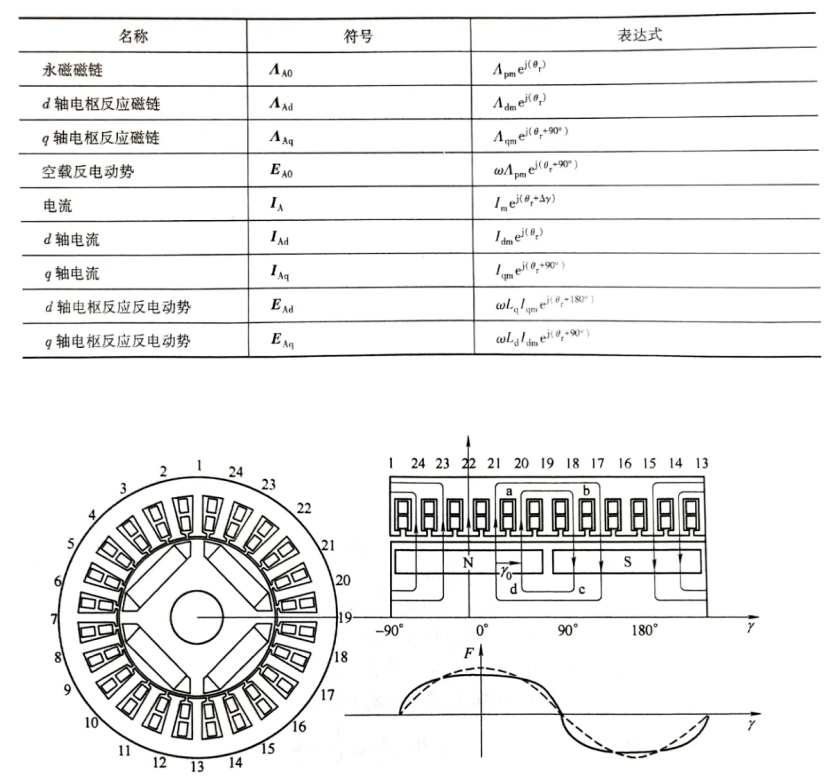
\includegraphics[width=1\linewidth]{./img/fig32.png}
  \caption{电机转子磁动势产生示意图}
\end{figure}

$$\left.\therefore\left\{\begin{array}{l}f_A=CNi_A\cos(\omega t+\alpha)\cos\gamma\\f_B=CNi_B\cos\left(\omega t+\alpha-120^\circ\right)\cos\left(\gamma-120^\circ\right)\\f_C=CNi_A\cos\left(\omega t+\alpha-240^\circ\right)\cos\left(\gamma-240^\circ\right)\end{array}\right.\right.$$

$$\therefore f_{s1}=f_A+f_B+f_C$$
$$=\frac{3C}{2}NI_m\cos[\gamma-(\omega t+\alpha)]=F_{s1}\cos[\gamma-(\omega t+\alpha)]$$

可以将定子绕组的合成电动势$f_{s1}$分解为直轴分量$f_{sd}$和交轴分量$f_{sq}$:($\Delta\gamma$为转矩角)。

$$\begin{aligned}
  &f_{s1} \begin{aligned}=F_{s1}\cos[\gamma-(\omega t+\alpha)]=F_{s1}\cos{[\gamma-(\theta_{r}+\Delta\gamma)]}\end{aligned}  \\
  &f_{s1} \begin{aligned}=F_{s1}\left[\cos(\Delta\gamma)\cos{(\gamma-\theta_{r})}-\sin(\Delta\gamma)\sin{(\gamma-\theta_{r})}\right]\end{aligned}  \\
  &f_{s1} \begin{aligned}=F_{s1}\cos(\Delta\gamma)\cos{(\gamma-\theta_{r})}+F_{s1}\sin(\Delta\gamma)\cos{[\gamma-(\theta_{r}+90^{\circ})]}\end{aligned} 
  \end{aligned}$$

定子绕组合成电动势分解

$$\left.\left\{\begin{array}{l}F_{sd}=|F_{sd}|e^{j(\theta_r)}=F_{s1}\cos(\Delta\gamma)e^{j(\theta_r)}\\F_{sq}=|F_{sq}|e^{j(\theta_r+90^{\circ})}=F_{s1}\cos(\Delta\gamma)e^{j(\theta_r+90^{\circ})}\\F_{s1}=F_{sd}+F_{sq}\end{array}\right.\right.$$
$$\left.\left\{\begin{array}{l}f_{sd}=F_{s1}\cos(\Delta\gamma)\cos{(\gamma-\theta_r)}\\f_{sq}=F_{s1}\sin(\Delta\gamma)\cos{[\gamma-(\theta_r+90^\circ)]}\\f_{s1}=f_{sd}+f_{sq}\end{array}\right.\right.$$

\subsubsection{电压电流波形展示}
% 插入电压电流等波形图片
\begin{figure}[H]
  \centering
  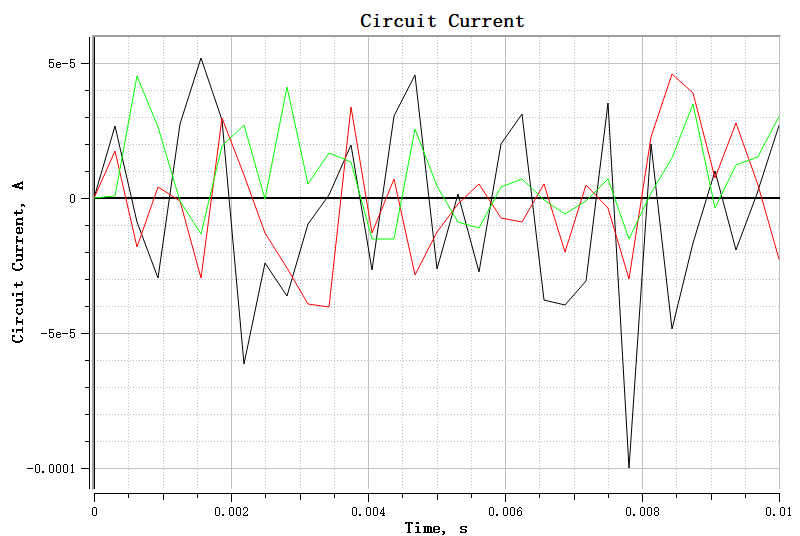
\includegraphics[width=1\linewidth]{./img/task1/noload-current.png}
  \caption{空载电流-接近0}
\end{figure}

\begin{figure}[H]
  \centering
  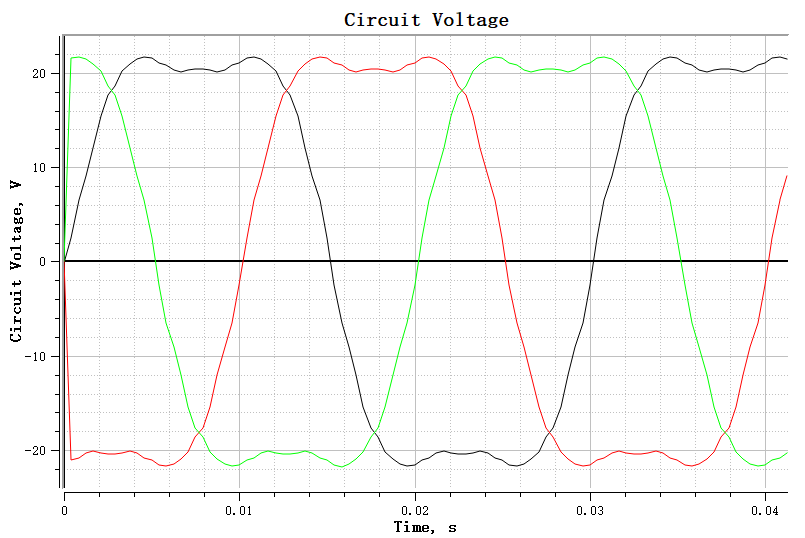
\includegraphics[width=1\linewidth]{./img/task1/noload-voltage.png}
  \caption{空载电流-接近0}
\end{figure}

\subsubsection{电机损耗展示}
% 插入两张电机损耗图
\begin{figure}[H]
  \centering
  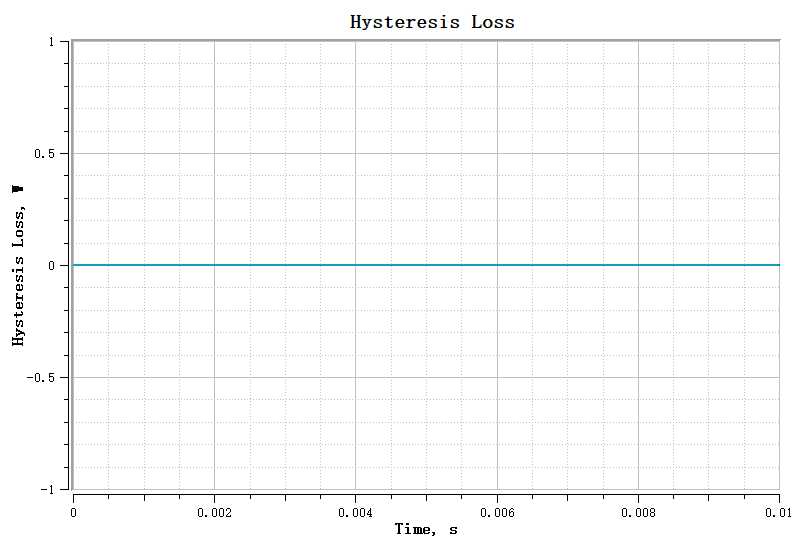
\includegraphics[width=1\linewidth]{./img/task1/noload-H-loss.png}
  \caption{空载情况下的焦耳损耗}
\end{figure}

\begin{figure}[H]
  \centering
  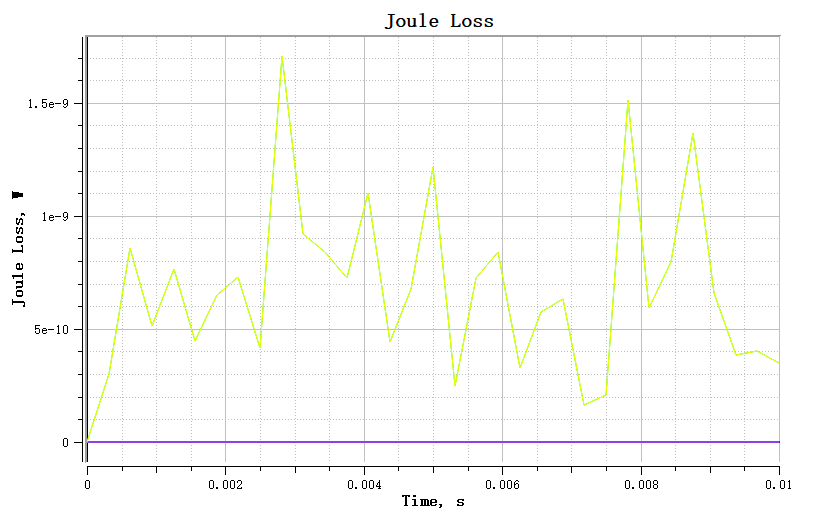
\includegraphics[width=1\linewidth]{./img/task1/noload-Joule-Loss.png}
  \caption{空载情况下的磁滞损耗}
\end{figure}

\subsection{转矩}
\subsubsection{推导}
根据能量守恒推导出电机转矩,推导过程中忽略了电阻项且近似认为系统的效率为1。
$$\begin{aligned}
  &P=3U_{A}I_{A}\operatorname{cos}\phi   \\
  & P=3U_{A}I_{A}\operatorname{cos}(\Delta\gamma+\phi-\Delta\gamma)  \\
  & P=3U_{A}I_{A}\operatorname{cos}(\Delta\gamma+\phi)\operatorname{cos}(\Delta\gamma)+3U_{A}I_{A}\operatorname{sin}(\Delta\gamma+\phi)\operatorname{sin}(\Delta\gamma)  \\
  & P=3\left(U_{d}I_{d}+U_{q}I_{q}\right)  \\
  &P=3\left[\left(E_{A0}+X_{d}I_{d}\right)I_{q}-X_{q}I_{q}I_{d}\right] \\
  &P=3\omega\left\{\left[\Lambda_{pm}+L_{d}I_{m}\operatorname{cos}(\Delta\gamma)\right]I_{m}\operatorname{sin}(\Delta\gamma)-I_{m}\operatorname{sin}(\Delta\gamma)\operatorname{cos}(\Delta\gamma)\right\} \\
  &P=3\omega\left[\Lambda_{pm}I_{m}\operatorname{sin}(\Delta\gamma)-\frac{(L_{q}-L_{d})I_{m}^{2}}2\operatorname{sin}(2\Delta\gamma)\right] \\
  &T_{m}=\frac{P}{\omega_{m}}=\frac{p}{2}\frac{P}{\omega}=\frac{3}{2}p\left[\Lambda_{pm}I_{m}\sin(\Delta\gamma)-\frac{(L_{q}-L_{d})I_{m}^{2}}{2}\sin(2\Delta\gamma)\right]
  \end{aligned}$$

转矩由两部分构成:第一部分只和永磁磁链有关,称为永磁转矩;第二部分与永磁无关,只和直交轴的电
感差值(即和直交轴磁阻差值)有关,称为磁阻转矩。永磁转矩在转矩角等于90°时取得最大值,而磁阻转矩
在转矩角为45°和135°时取得最大值。总转矩最大值的转矩角则与电机参数有关。

\subsubsection{空载转矩仿真图}
\begin{figure}[H]
  \centering
  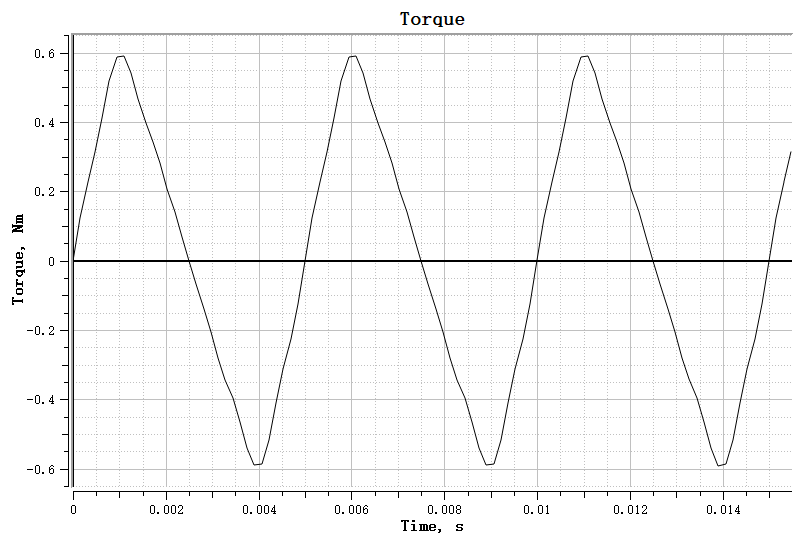
\includegraphics[width=1\linewidth]{./img/task1/noload-torque.png}
  \caption{空载情况下的转矩}
\end{figure}

%%=========================================================================
\section{Task2:绕组结构对比}
考虑三种不同的绕组方式:y=1(集中绕组),y=2(短距绕组),y=3(整距绕组)。
这三种绕组方式的区别主要体现在绕组的分布上面,具体如下:

1)y=1 集中绕组

\begin{itemize}
	\item 在集中绕组中,同一相的所有线圈都集中在相邻的几个槽内。
	\item 这种绕组方式简单,制造成本较低。
	\item 但其缺点是谐波含量较高,可能导致电机效率和平滑运行性能下降。
\end{itemize}
\begin{figure}[H]
  \centering
  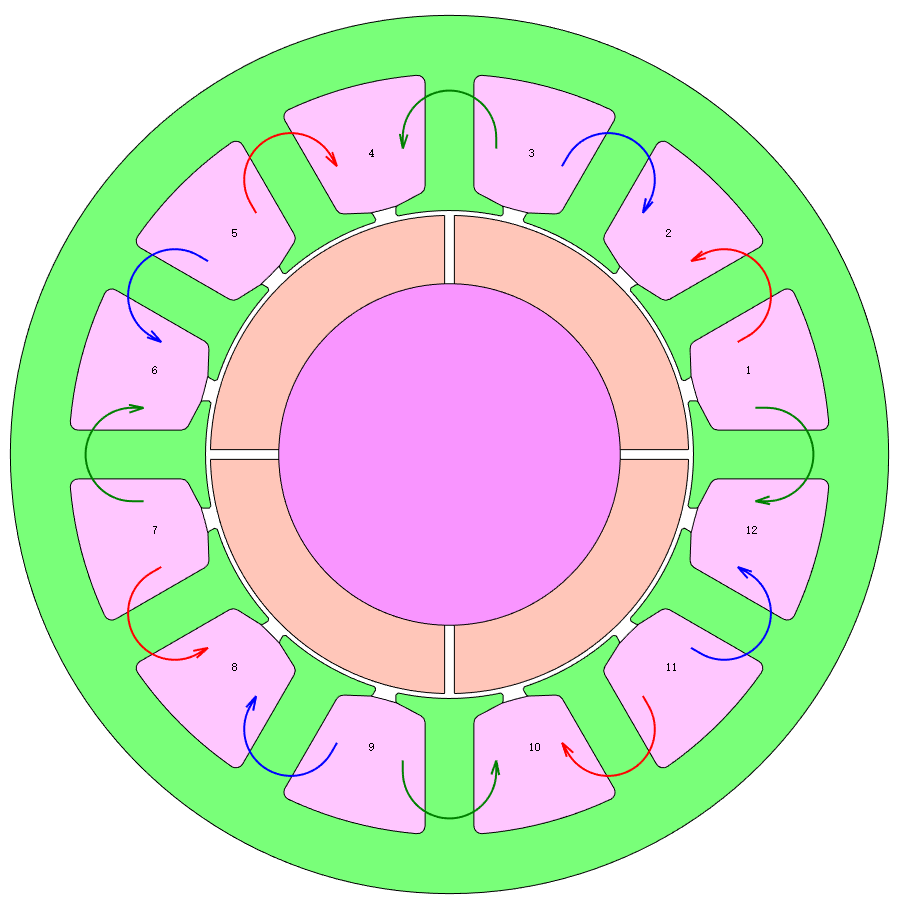
\includegraphics[width=1\linewidth]{./img/task2/model1.png}
  \caption{$y=1$}
\end{figure}

2)y=2 短距绕组

\begin{itemize}
	\item 短距绕组是一种折衷方案,其中线圈分布在稍微分散的槽中,但不像整距绕组那样完全分散。
	\item 这种绕组方式可以减少谐波影响,提高电机效率和运行平滑性。
	\item 制造复杂度和成本介于集中绕组和整距绕组之间。
\end{itemize}
\begin{figure}[H]
  \centering
  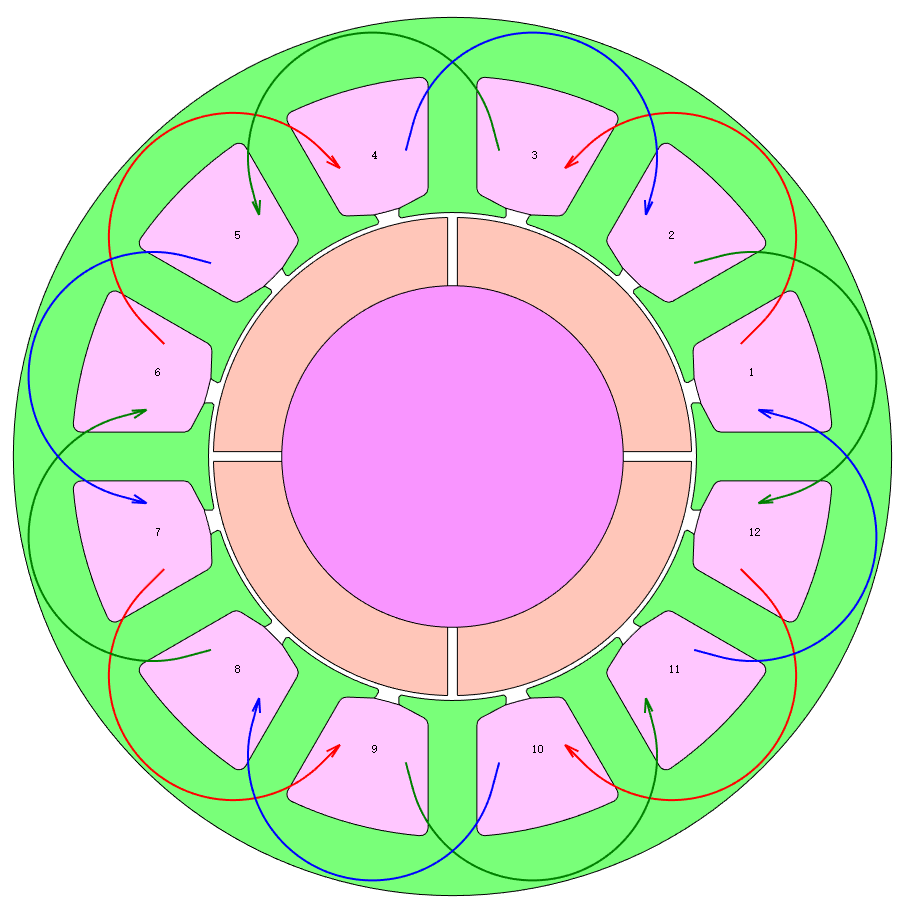
\includegraphics[width=1\linewidth]{./img/task2/model2.png}
  \caption{$y=2$}
\end{figure}

3) y=3 整距绕组

\begin{itemize}
	\item 整距绕组中,线圈均匀分布在所有的槽中。
	\item 这种方式可以极大地减少谐波,提高电机的效率和运行性能。
	\item 制造过程更为复杂,成本更高。
\end{itemize}
\begin{figure}[H]
  \centering
  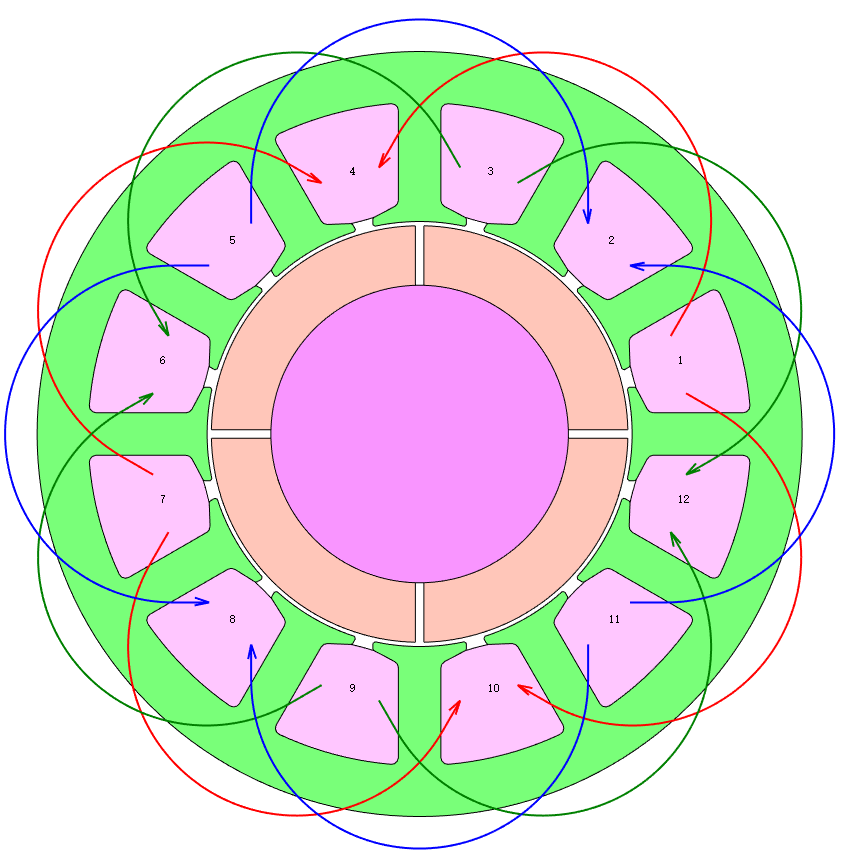
\includegraphics[width=1\linewidth]{./img/task2/model3.png}
  \caption{$y=3$}
\end{figure}

\subsection{空载性能对比}

\subsubsection{转矩}
经过观察并分析以下三幅图可以得知
\begin{itemize}
	\item 集中绕组:产生较大的峰值转矩;转矩脉动较大,可能会导致机械振动和噪音。
	\item 短距绕组:转矩介于集中绕组和整距绕组之间;转矩脉动低于集中绕组但高于整距绕组。
	\item 整距绕组:平滑的转矩曲线,但峰值转矩可能低于集中绕组;同时拥有最小的转矩脉动,可以为电机带来更平稳的运行。
\end{itemize}

\begin{figure}[H]
  \centering
  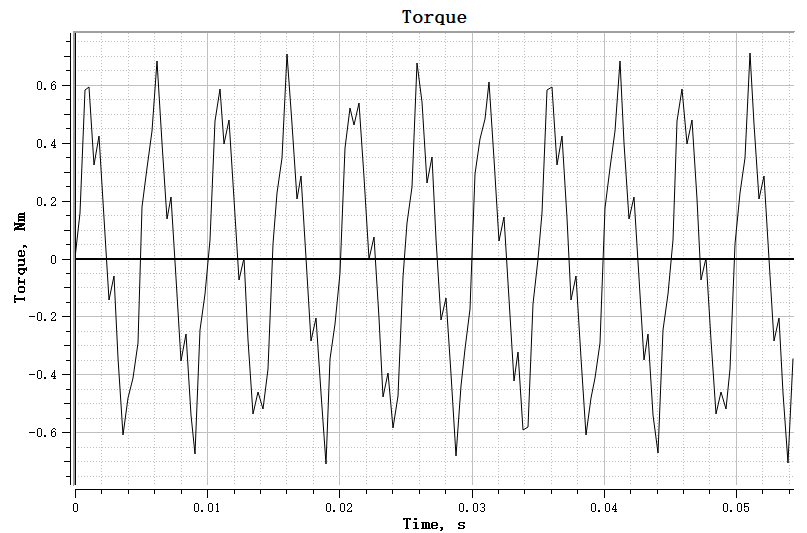
\includegraphics[width=1\linewidth]{./img/task2/torque-y1.png}
  \caption{$y=1$}
\end{figure}
\begin{figure}[H]
  \centering
  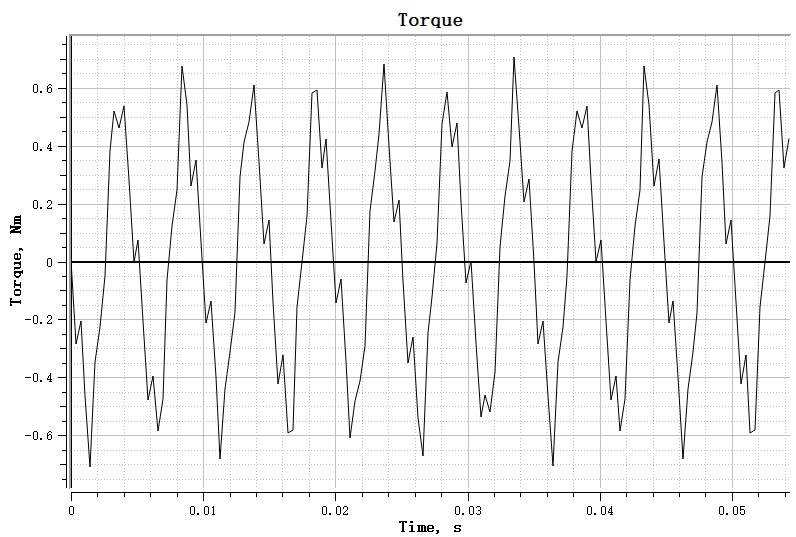
\includegraphics[width=1\linewidth]{./img/task2/torque-y2.png}
  \caption{$y=2$}
\end{figure}
\begin{figure}[H]
  \centering
  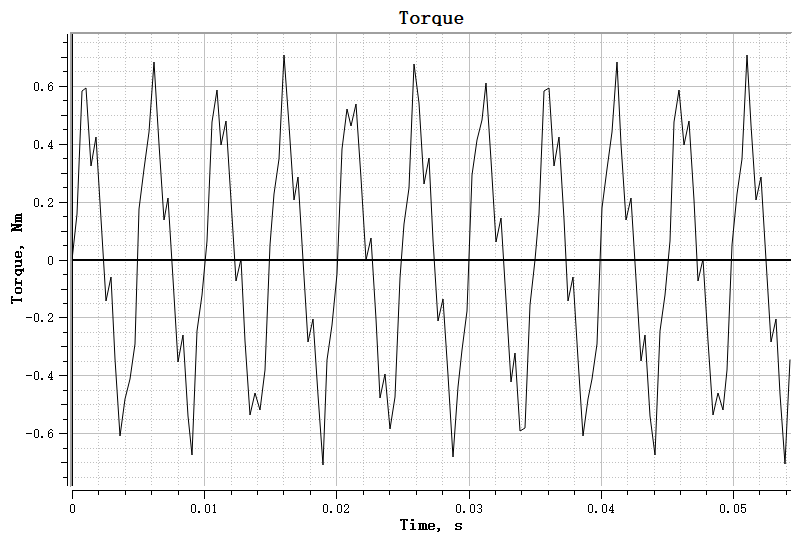
\includegraphics[width=1\linewidth]{./img/task2/torque-y3.png}
  \caption{$y=3$}
\end{figure}

\subsubsection{反电势}
\begin{figure}[H]
  \centering
  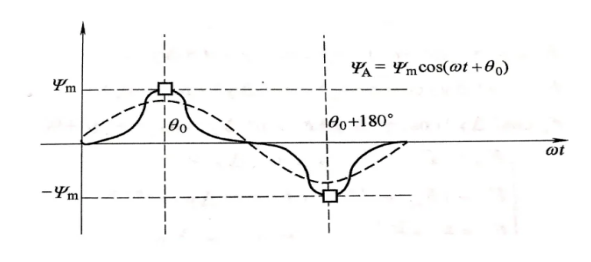
\includegraphics[width=1\linewidth]{./img/task2/flux.png}
  \caption{A相磁链波形}
\end{figure}

$A/B/C$三相绕组的轴线分别位于$\gamma$等于
0、120、和240处。因此从A相磁链波形图中可以得
知,转子再转过$\theta_0$时,转子磁动势的波峰将对准A相
绕组轴线,A相绕组匝链的磁通量取得最大值;转子再
转过$\theta_0 + 180$时,转子磁动势的波谷将对准A相绕组
轴线,A相绕组匝链的硒通量取得最小值。该值与最大
值大小相等,方向相反。将波形进行谐波分解可以得到
其基波分量(如图中虚线所示)。三相定子绕组的磁动
势基波分量可以通过下列方程式表示:
$$\left.\left\{\begin{array}{l}\psi_{A0}=\psi_{m0}\cos\left(\omega t+\theta_0\right)=\psi_{m0}\cos\left(\theta_r\right)\\\psi_{B0}=\psi_{m0}\cos\left(\omega t+\theta_0-120^\circ\right)=\psi_{m0}\cos\left(\theta_r-120^\circ\right)\\\psi_{C0}=\psi_{m0}\cos\left(\omega t+\theta_0-240^\circ\right)=\psi_{m0}\cos\left(\theta_r-240^\circ\right)\end{array}\right.\right.$$
根据法拉第电磁感应定律,将磁链进行求导即可得到空载反电动势的表达式:
$$\left.\left\{\begin{array}{l}e_{A0}=\frac{d}{dt}\psi_{A0}=\omega\psi_{m0}\cos{(\theta_r+90^\circ)}\\e_{B0}=\frac{d}{dt}\psi_{B0}=\omega\psi_{m0}\cos{(\theta_r+90^\circ-120^\circ)}\\e_{C0}=\frac{d}{dt}\psi_{C0}=\omega\psi_{m0}\cos{(\theta_r+90^\circ-240^\circ)}\end{array}\right.\right.$$
将以上的磁动势与空载反电动势使用向量表示:
$$\left.\left\{\begin{array}{l}\dot{\psi}_{A0}=\dot{\psi}_{m0}e^{j(\theta_r)}\\\dot{E}_{A0}=\mathrm{j}\omega\dot{\psi}_{A0}=\omega\dot{\psi}_{m0}e^{j(\theta_r+90\text{o})}\end{array}\right.\right.$$

\begin{figure}[H]
  \centering
  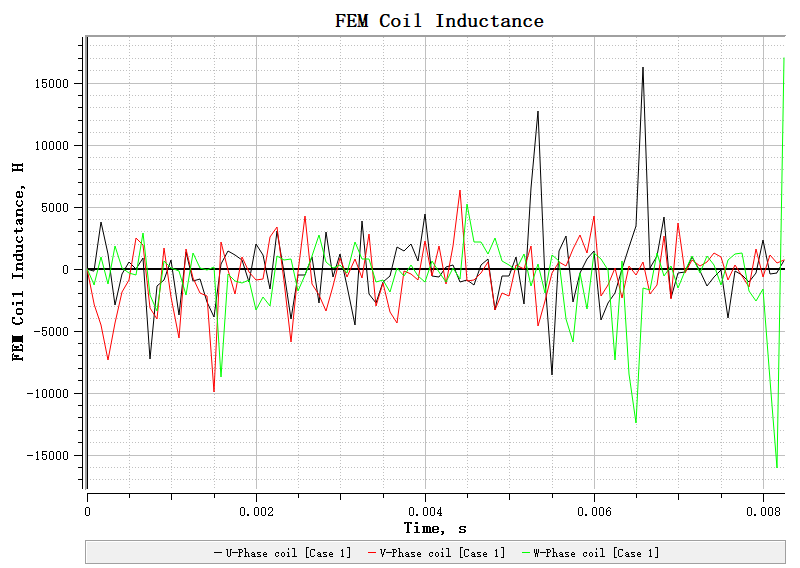
\includegraphics[width=1\linewidth]{./img/task2/FEM-y1.png}
  \caption{空载反电势,$y=1$}
\end{figure}
\begin{figure}[H]
  \centering
  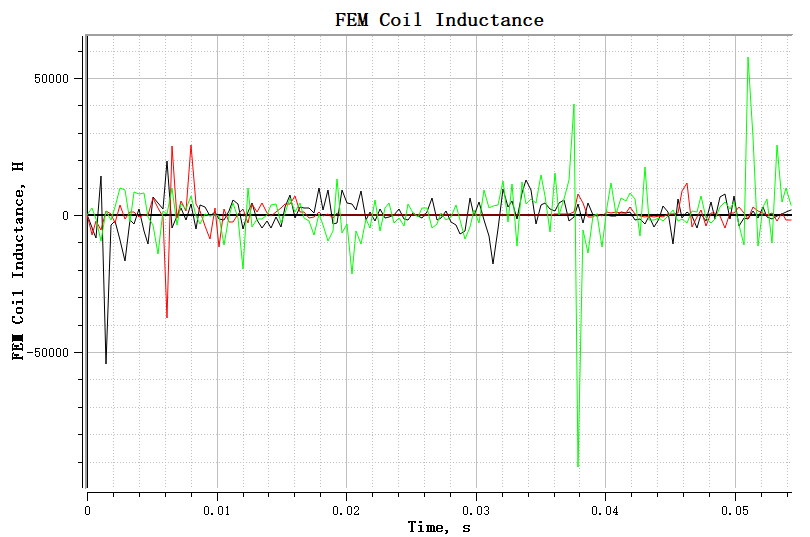
\includegraphics[width=1\linewidth]{./img/task2/FEM-y2.png}
  \caption{空载反电势,$y=2$}
\end{figure}
\begin{figure}[H]
  \centering
  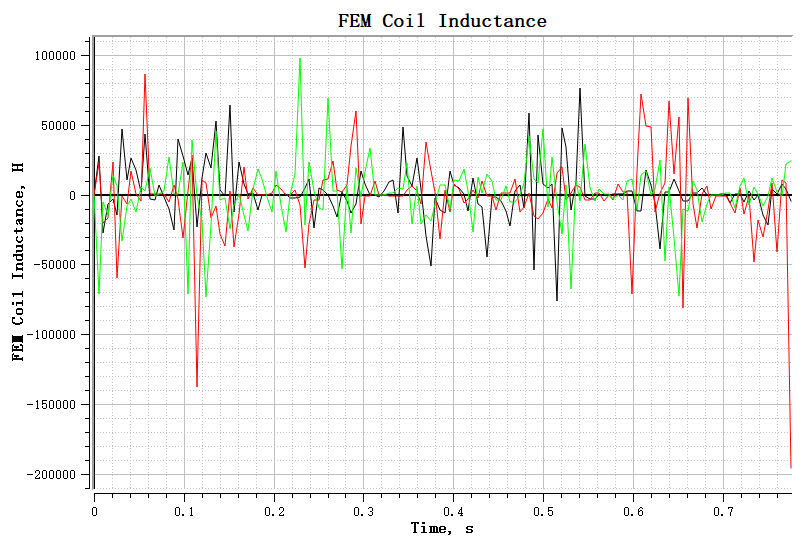
\includegraphics[width=1\linewidth]{./img/task2/FEM-y3.png}
  \caption{空载反电势,$y=3$}
\end{figure}
观察并分析得:

1. 空载反电势
\begin{itemize}
	\item 集中绕组(y=1):通常产生较高的空载反电势。波形可能更接近方波,这可能导致更高的谐波含量。
	\item 短距绕组(y=2):反电势波形会介于集中绕组和整距绕组之间,谐波含量较集中绕组低,但高于整距绕组。
	\item 整距绕组(y=3):产生较平滑的反电势波形,谐波含量最低,接近正弦波。
\end{itemize}

2. 反电势谐波
\begin{itemize}
	\item 集中绕组:谐波含量较高,可能会导致更多的噪声和振动。
	\item 短距绕组:谐波含量低于集中绕组但高于整距绕组,平衡了效率和噪声/振动。
	\item 整距绕组:最低的谐波含量,导致更低的噪声和振动。
\end{itemize}

\subsubsection{磁滞损耗}
磁滞损耗是由于材料内部磁畴重新排列时产生的能量损失。
使用的铁芯材料的磁滞特性决定了磁滞损耗的大小。
软磁材料,如硅钢,通常具有较低的磁滞损耗。
磁滞损耗随着频率的增加而增加。在高速运行的电机中,磁滞损耗可能变得更加显著。

\begin{figure}[H]
  \centering
  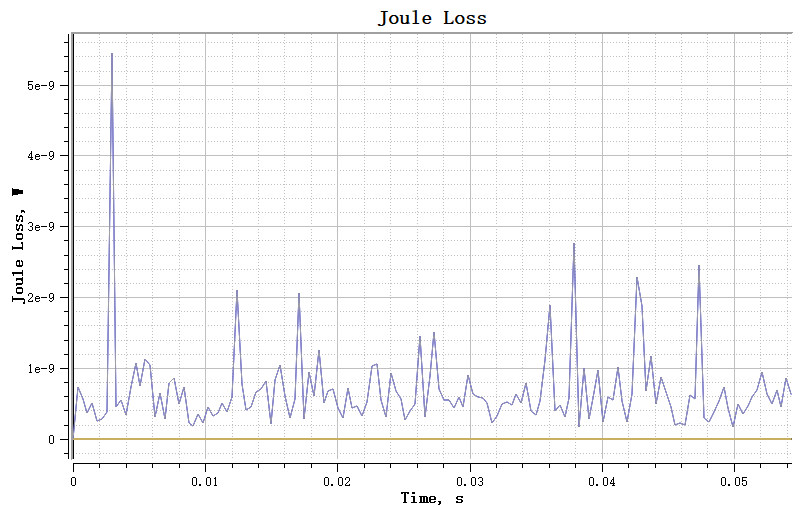
\includegraphics[width=1\linewidth]{./img/task2/joule-y1.png}
  \caption{空载条件下的磁滞损耗,$y=1$}
\end{figure}
\begin{figure}[H]
  \centering
  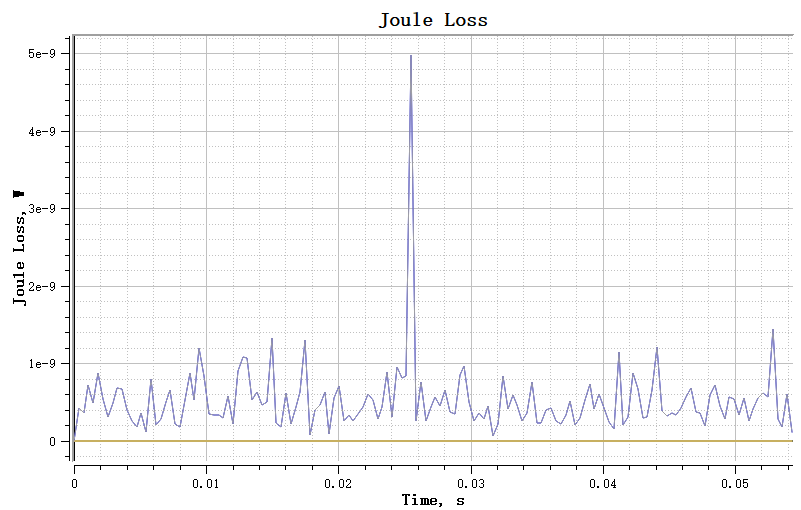
\includegraphics[width=1\linewidth]{./img/task2/joule-y2.png}
  \caption{空载条件下的磁滞损耗,$y=2$}
\end{figure}
\begin{figure}[H]
  \centering
  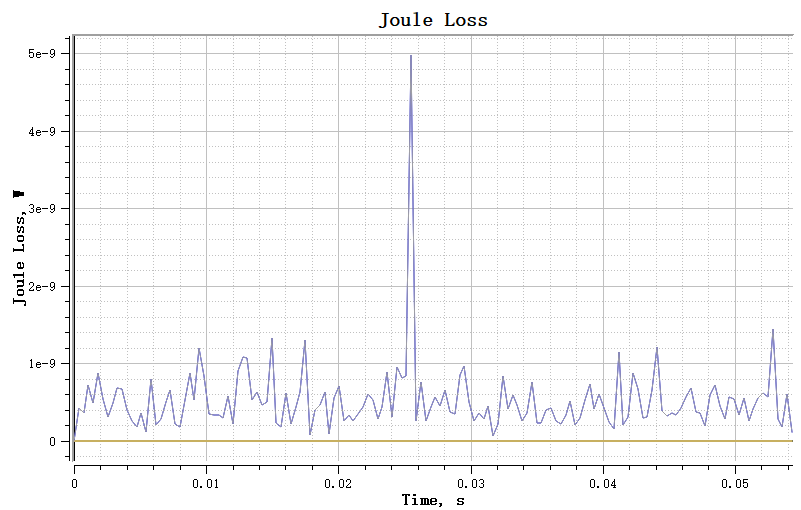
\includegraphics[width=1\linewidth]{./img/task2/joule-y2.png}
  \caption{空载条件下的磁滞损耗,$y=3$}
\end{figure}
对比可以看出:
\begin{itemize}
	\item 集中绕组:由于磁通分布不均匀,可能导致局部磁饱和和增加的磁滞损耗。
	\item 短距绕组:磁通分布比集中绕组更均匀,磁滞损耗低于集中绕组但高于整距绕组。
	\item 整距绕组:最均匀的磁通分布,因此磁滞损耗最低。
\end{itemize}


\subsection{负载性能对比}

用电流源模拟负载,电流源模型参数如下:
\begin{figure}[H]
  \centering
  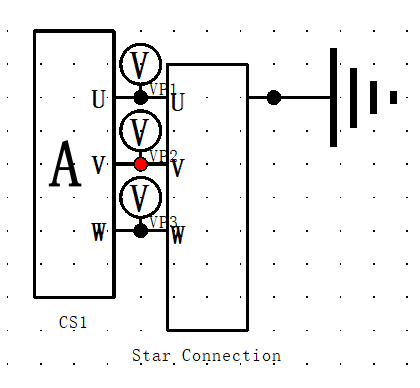
\includegraphics[width=0.8\linewidth]{./img/task2/load.png}
  \caption{负载条件下的电路图}
\end{figure}
\begin{figure}[H]
  \centering
  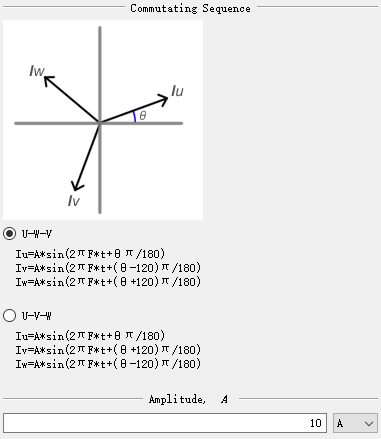
\includegraphics[width=0.8\linewidth]{./img/task2/load-config.png}
  \caption{电流源参数配置(峰值10A)}
\end{figure}

\subsubsection{电压}
当电机负载增加时,由于电阻和感抗的作用,电压会有所降落。
适当的绕组设计和选用适当的电缆和接触器可以减少电压损失。
\begin{figure}[H]
  \centering
  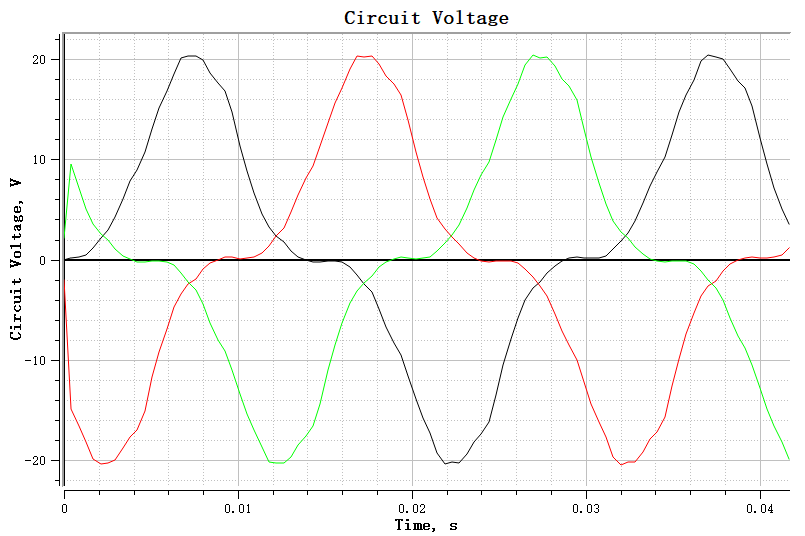
\includegraphics[width=1\linewidth]{./img/task2/voltage-y1-load.png}
  \caption{负载条件下的电压波形,$y=1$}
\end{figure}
\begin{figure}[H]
  \centering
  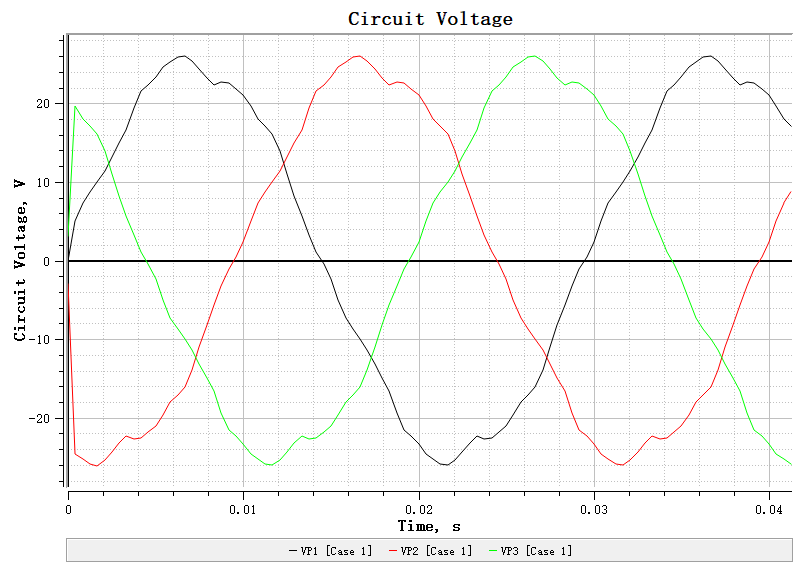
\includegraphics[width=1\linewidth]{./img/task2/voltage-y2-load.png}
  \caption{负载条件下的电压波形,$y=2$}
\end{figure}
\begin{figure}[H]
  \centering
  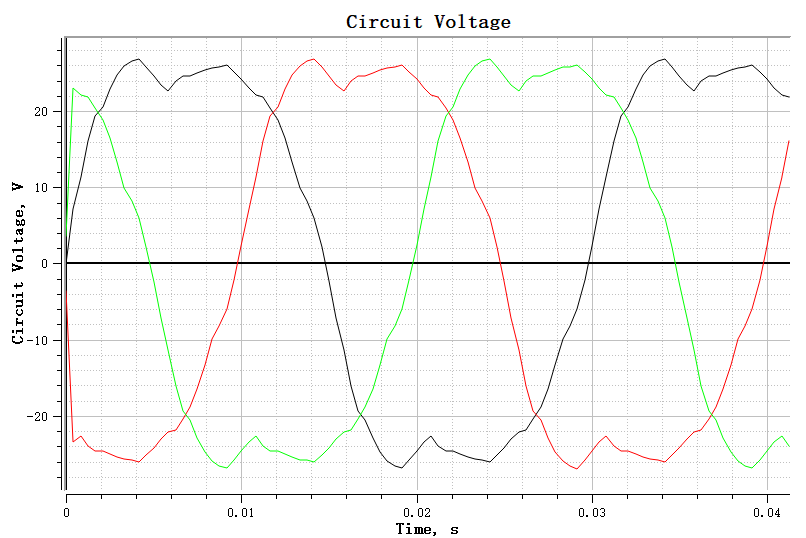
\includegraphics[width=1\linewidth]{./img/task2/voltage-y3-load.png}
  \caption{负载条件下的电压波形,$y=3$}
\end{figure}
经过观察可以发现:

集中绕组、短距绕组、整距绕组的波动依次减小,在峰值电压处保留的时间逐渐变长,显示出了很好的稳定性。

具体来讲:
\begin{itemize}
	\item 集中绕组:可能由于绕组的不均匀分布导致电压分布不均,尤其在高负载情况下。
	\item 短距绕组:比集中绕组有更好的电压均衡性能,但仍然不如整距绕组。
	\item 整距绕组:提供最佳的电压均衡,尤其在高负载下。
\end{itemize}

\subsubsection{反电势}
反电势的变化主要来源于:负载增加会导致反电势减少。
这是因为反电势与转速和磁通量成比例,而负载会影响电机的转速。

调节:通过调节控制器和电源,可以对反电势的变化进行补偿,保持电机性能的稳定。

\begin{figure}[H]
  \centering
  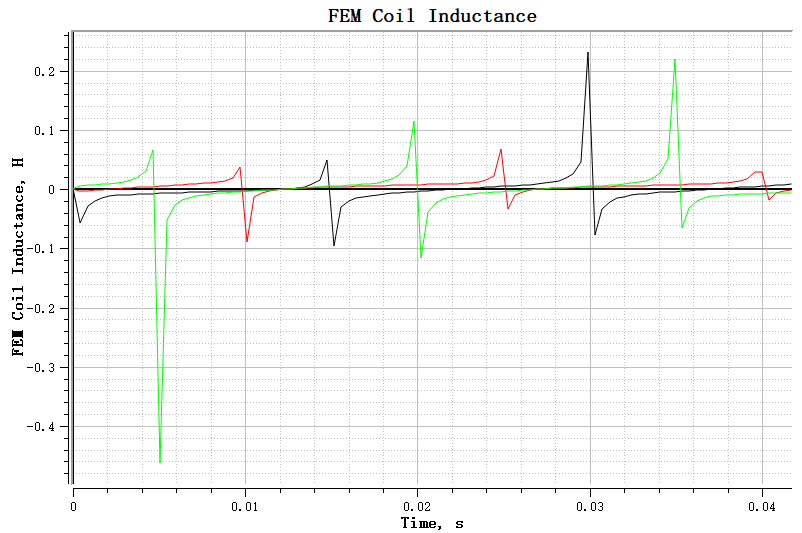
\includegraphics[width=1\linewidth]{./img/task2/FEM-y1-load.png}
  \caption{负载条件下的反电势波形,$y=1$}
\end{figure}
\begin{figure}[H]
  \centering
  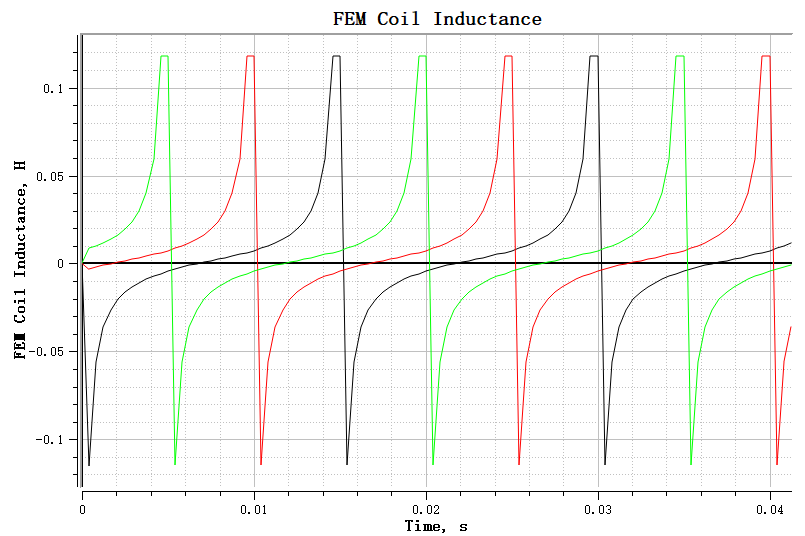
\includegraphics[width=1\linewidth]{./img/task2/FEM-y2-load.png}
  \caption{负载条件下的反电势波形,$y=2$}
\end{figure}
\begin{figure}[H]
  \centering
  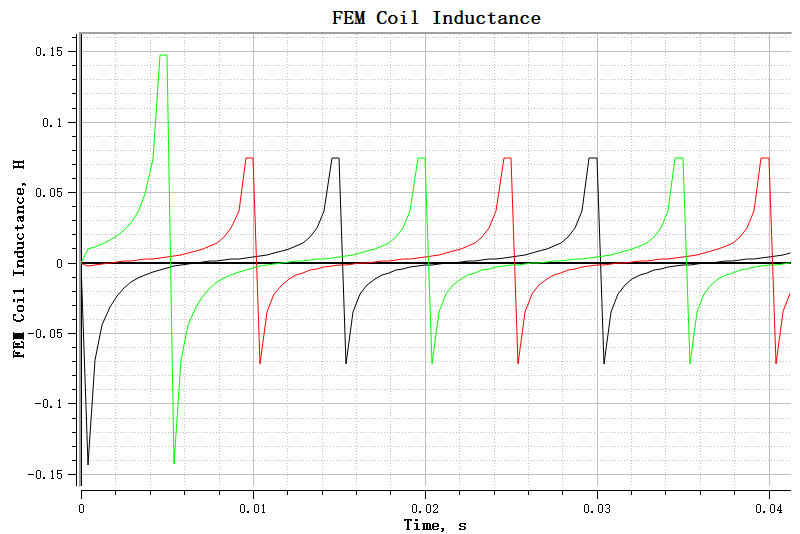
\includegraphics[width=1\linewidth]{./img/task2/FEM-y3-load.png}
  \caption{负载条件下的反电势波形,$y=3$}
\end{figure}

对比以上三幅波形图可以看出:

\begin{itemize}
	\item 集中绕组:因绕组不均匀导致反电势波动大。
	\item 短距绕组:反电势波动小于集中绕组,但大于整距绕组。
	\item 整距绕组:因为磁通分布均匀,所以反电势最稳定。
\end{itemize}

\subsubsection{转矩}

转矩波动来源:负载是以正弦电流的形式加载,负载增加意味着需要更大的转矩来克服负载。

改变转矩的方法主要有以下三个:

绕组电流:提高电流可以增加转矩。

永磁体特性:强磁场可以提供更大的转矩。

转矩特性:理想情况下,转矩与电流成线性关系,因此调整电机中的电流可以在一定程度上影响转矩。

\begin{figure}[H]
  \centering
  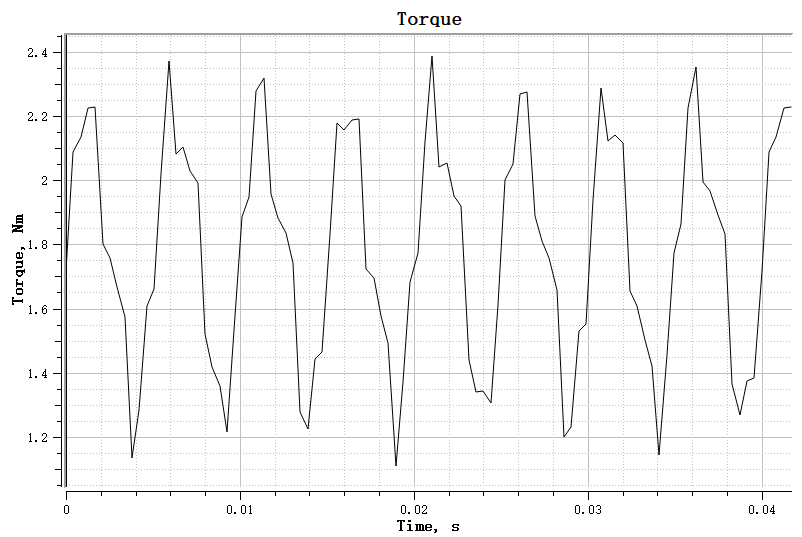
\includegraphics[width=1\linewidth]{./img/task2/torque-y1-load.png}
  \caption{负载条件下的转矩,$y=1$}
\end{figure}
\begin{figure}[H]
  \centering
  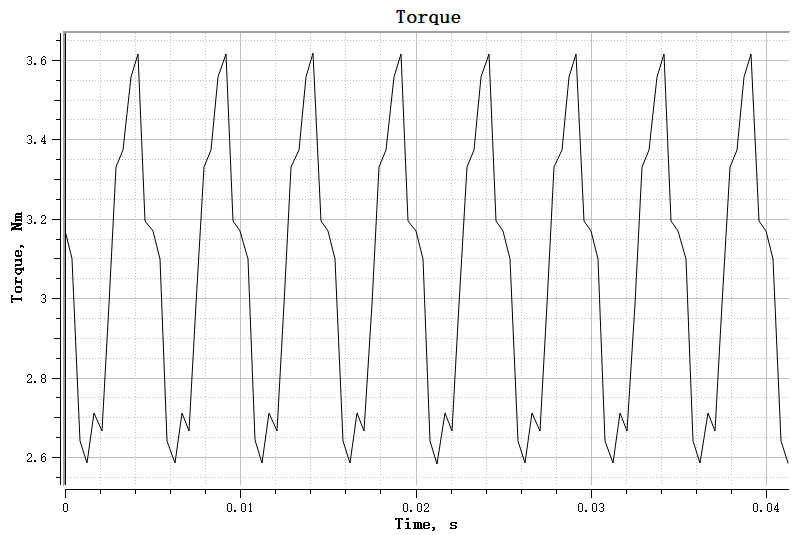
\includegraphics[width=1\linewidth]{./img/task2/torque-y2-load.png}
  \caption{负载条件下的转矩,$y=2$}
\end{figure}
\begin{figure}[H]
  \centering
  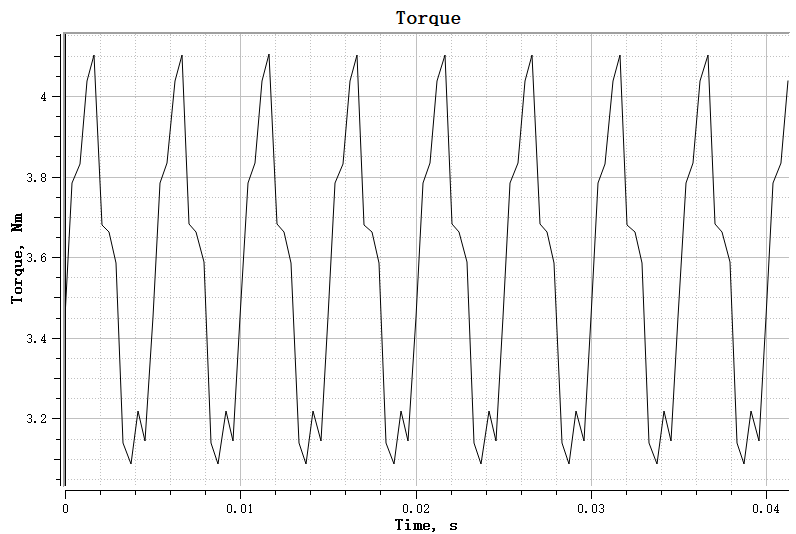
\includegraphics[width=1\linewidth]{./img/task2/torque-y3-load.png}
  \caption{负载条件下的转矩,$y=3$}
\end{figure}

对比,观察可得:
\begin{itemize}
	\item 集中绕组:产生较大的峰值转矩,但转矩脉动也大,可能导致噪音和振动。
	\item 短距绕组:转矩平稳性比集中绕组好,但不如整距绕组。
	\item 整距绕组:提供最平稳的转矩输出,转矩脉动最小。
\end{itemize}


\subsubsection{电力输出}

电力输出可以通过电压和电流的乘积计算得出。
在较高的负载下,电机效率可能降低,因为损耗(如铜损、铁损)相对于输出功率占比增加。

\begin{figure}[H]
  \centering
  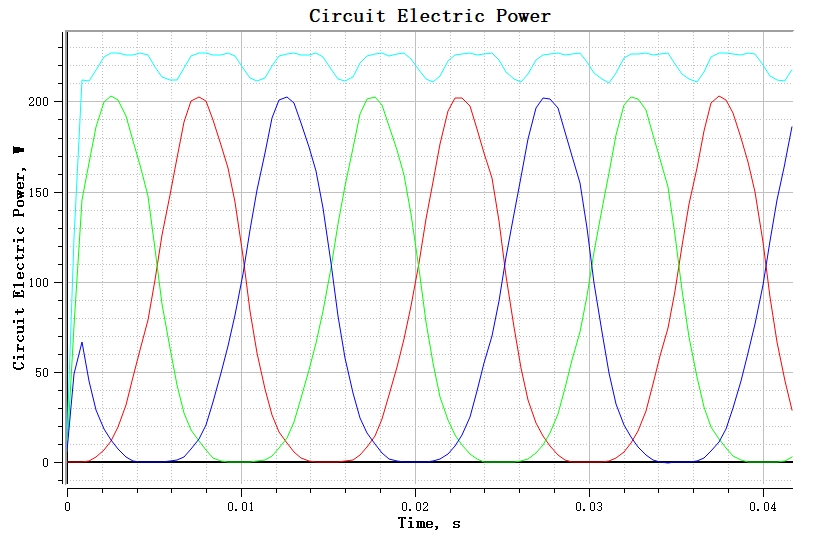
\includegraphics[width=1\linewidth]{./img/task2/power-y1-load.png}
  \caption{负载条件下的电力输出,$y=1$}
\end{figure}
\begin{figure}[H]
  \centering
  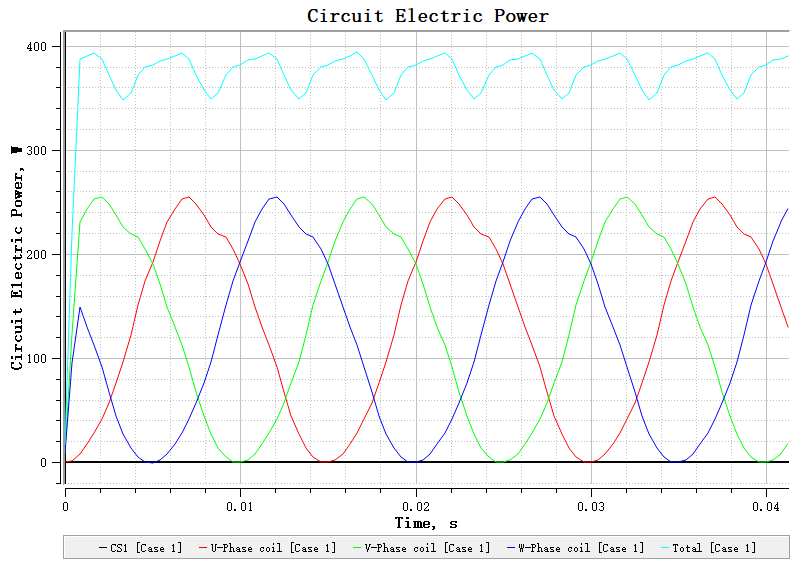
\includegraphics[width=1\linewidth]{./img/task2/power-y2-load.png}
  \caption{负载条件下的电力输出,$y=2$}
\end{figure}
\begin{figure}[H]
  \centering
  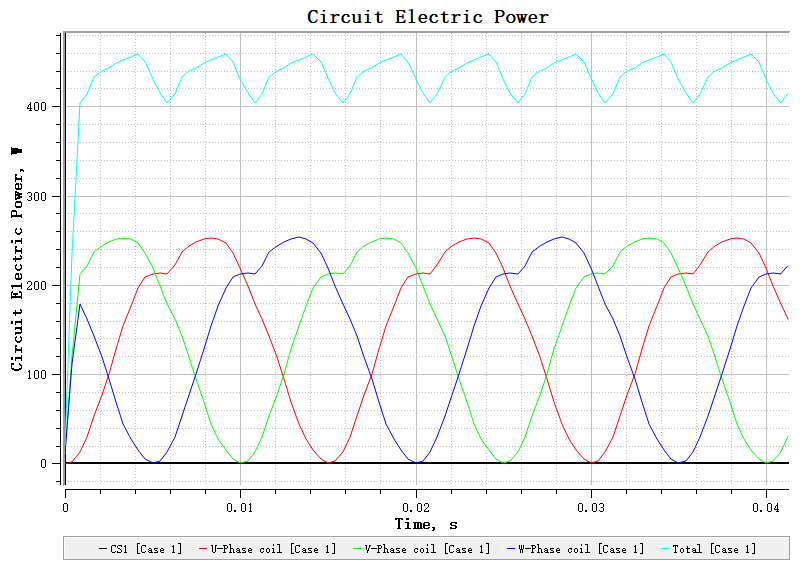
\includegraphics[width=1\linewidth]{./img/task2/power-y3-load.png}
  \caption{负载条件下的电力输出,$y=3$}
\end{figure}

\begin{itemize}
	\item 集中绕组:由于转矩脉动和电压不均匀性,可能导致电力输出不稳定。
	\item 短距绕组:在电力输出稳定性方面比集中绕组好,但不如整距绕组。
	\item 整距绕组:因为有最好的转矩平稳性和电压均衡,所以提供最稳定的电力输出。
\end{itemize}
此外,随着y值的上升,电力输出功率整体呈现上升趋势。

\subsection{绕组结构对比小结}
在选择三相永磁电机的绕组方式时,理解集中绕组、短距绕组和整距绕组各自的优势和劣势至关重要,因为每种方式都适用于不同的应用场景和性能需求。集中绕组由于其独特的绕组布局,通常能够提供较高的峰值转矩,这使得它适合于那些需要快速动态响应和高转矩密度的应用,如某些类型的电动工具或特殊的工业设备。然而,这种配置可能会引起较大的磁滞损耗和谐波干扰,这可能不适合对电磁兼容性有严格要求的应用。

另一方面,整距绕组因其更均匀的磁通分布,通常能够提供更平滑的运行性能,这包括较低的噪音、较小的振动以及更稳定的转矩输出。这种特性使得整距绕组非常适合于噪音和振动对设备性能和耐用性有显著影响的应用,例如精密仪器或需要安静运行的家用电器。

短距绕组则提供了一种介于集中绕组和整距绕组之间的解决方案。它在保持较好的转矩性能的同时,能够较好地控制噪音和振动,这使得它适合于那些既需要一定程度的动力输出,又要求电机运行相对平稳的应用场景,如某些商业和轻工业应用。

此外,不同绕组方式对电机的冷却效率、维护需求以及制造成本也有显著影响。集中绕组可能由于其结构和散热特性而更难冷却,而整距绕组则可能在制造过程中更为复杂和昂贵。因此,电机设计师需要根据特定应用的性能要求、成本限制以及维护和操作条件来权衡这些因素,以确定最佳的绕组配置。最终,正确的绕组选择可以显著提高电机的整体性能和效率,同时满足特定应用场景的严格要求。

% =======================================
\section{Task3: 极对数对比}
各个特性的特点以及影响因素都在Task1和Task2中有了详细的阐述,因此在这个部分就不再赘述了,直接进行对比分析。

对比分析4极、8极和10极电机模型时,我们主要关注的是这些电机在空载反电势、
反电势谐波、转矩和转矩脉动方面的性能差异。每种极数的电机有其独特的特性和适用场景。

其中,需要首先明确的是三种模型的转速差异:

电机的转速与其极对数之间存在直接关系。通常,电机的转速由其同步转速决定,
这是电机在无负载条件下理论上可以达到的最高转速,由电源频率和电机的极对数决定。
同步转速$N_s$可以用公式$N_s=\frac{120\times f}P$计算,其中f是电源频率,P是极对数。
\begin{itemize}
	\item 4极电机(2极对):由于极对数较少,这类电机的同步转速较高。在相同的电源频率下,4极电机会比8极或10极电机转得更快。
	\item 8极电机(4极对):具有更多的极对,因此其同步转速低于4极电机。这意味着在相同的电源频率下,8极电机的转速会减半。
	\item 10极电机(5极对):极对数更多,导致同步转速进一步降低。其转速将低于8极电机,是4极电机同步转速的大约五分之二。
\end{itemize}

\subsection{空载性能对比}
\subsubsection{转矩}
\begin{itemize}
	\item 4极电机:在空载条件下,4极电机的转矩通常较低,因为它们是为高速运行而设计的。空载转矩主要由电机的内部摩擦和空气阻力决定。
	\item 8极和10极电机:这些电机在空载条件下也会展现出较低的转矩,但由于它们的转速通常较低,因此空载损耗(如摩擦和空气阻力)相对更小。
\end{itemize}

\begin{figure}[H]
  \centering
  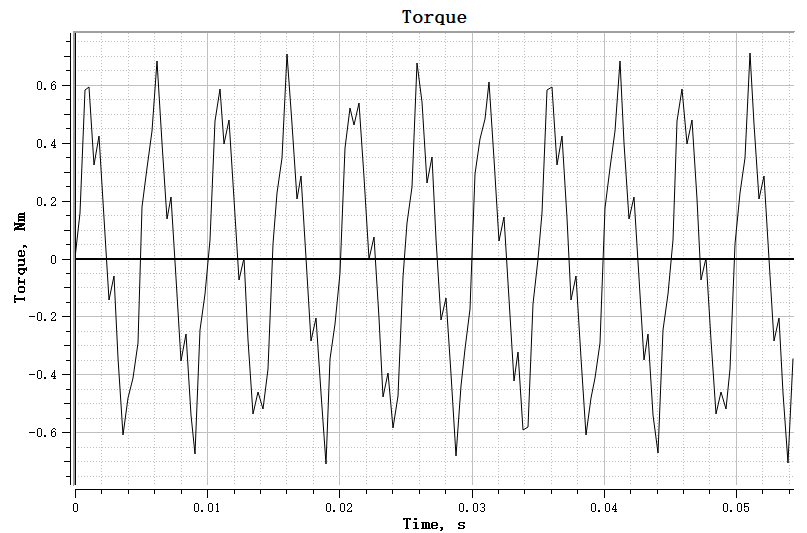
\includegraphics[width=1\linewidth]{./img/task3/torque-n4.png}
  \caption{$n=4$}
\end{figure}
\begin{figure}[H]
  \centering
  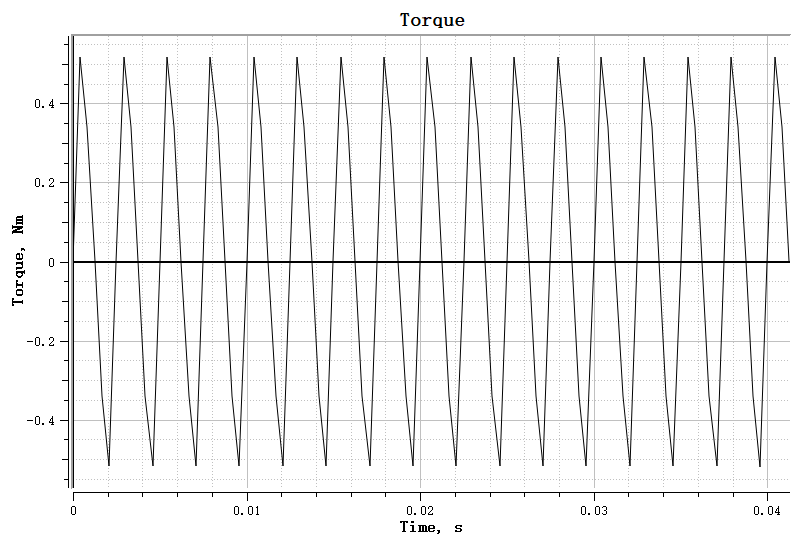
\includegraphics[width=1\linewidth]{./img/task3/torque-n8.png}
  \caption{$n=8$}
\end{figure}
\begin{figure}[H]
  \centering
  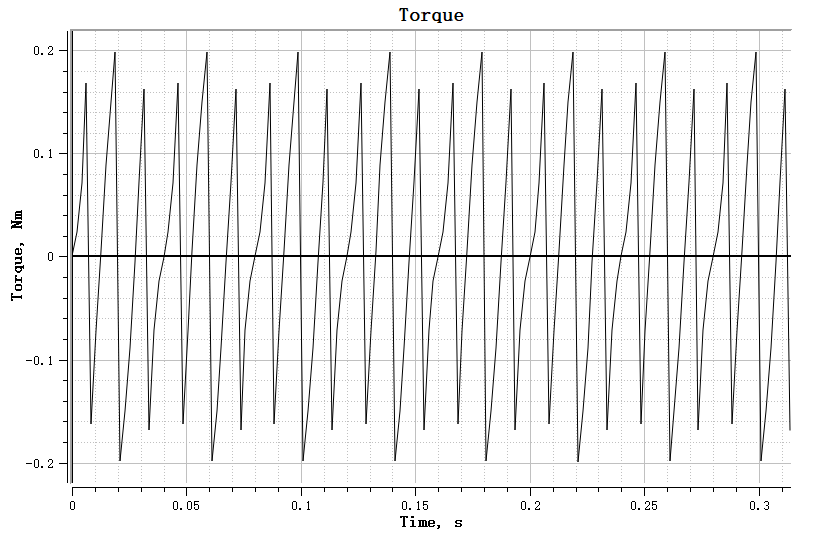
\includegraphics[width=1\linewidth]{./img/task3/torque-n10.png}
  \caption{$n=10$}
\end{figure}

\subsubsection{反电势}
在空载状态下的反电势方面,通过观察下面仿真得出的三张图可以明显的看出:
\begin{itemize}
	\item 4极电机:通常会有较高的空载反电势,因为每个极所需的转速更高。这意味着在相同的电机尺寸和磁场强度下,4极电机能够产生更高的电压。
	\item 8极和10极电机:由于更多的极数导致单个极的转速降低,这些电机的空载反电势相对较低。这使得它们适用于需要较低速度和较高扭矩密度的应用。
\end{itemize}

\begin{figure}[H]
  \centering
  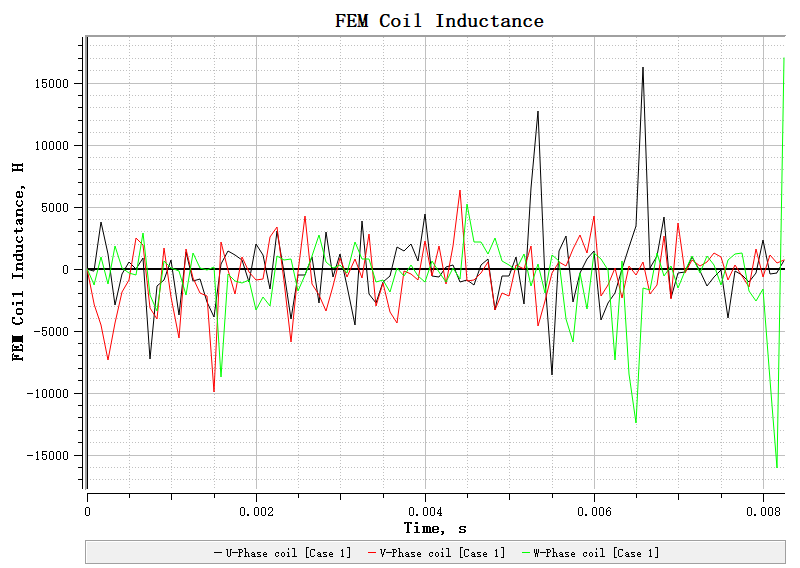
\includegraphics[width=1\linewidth]{./img/task3/FEM-n4.png}
  \caption{空载反电势,$n=4$}
\end{figure}
\begin{figure}[H]
  \centering
  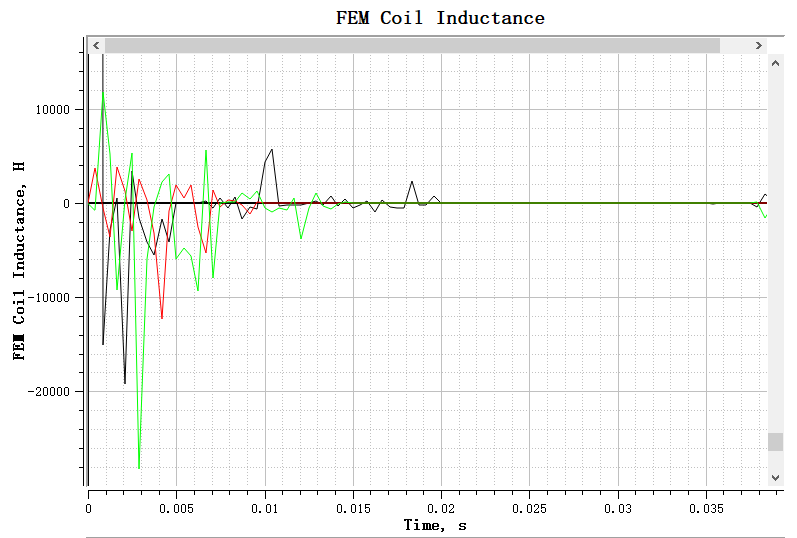
\includegraphics[width=1\linewidth]{./img/task3/FEM-n8.png}
  \caption{空载反电势,$n=8$}
\end{figure}
\begin{figure}[H]
  \centering
  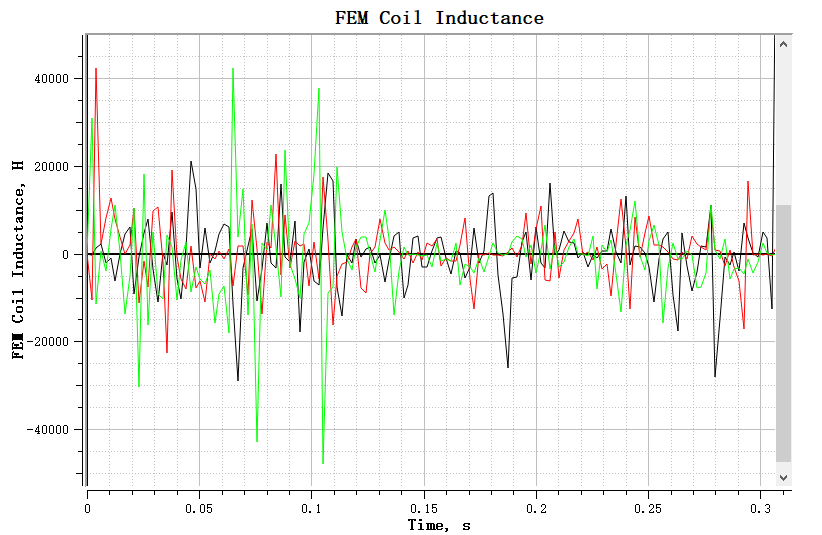
\includegraphics[width=1\linewidth]{./img/task3/FEM-n10.png}
  \caption{空载反电势,$n=10$}
\end{figure}

\subsubsection{磁滞损耗}
磁滞损耗是由于电机铁芯材料内部的磁畴在每个工作周期中重排引起的能量损失。
这种损耗与电机的工作频率和材料的磁滞特性有关。
\begin{itemize}
	\item 4极电机:通常工作在较高的频率下,这可能导致较高的磁滞损耗。然而,由于4极电机的设计通常更注重高速和高效,所使用的材料可能具有较低的磁滞损耗特性。
	\item 8极和10极电机:由于工作在较低的频率,理论上磁滞损耗会较低。但这也取决于使用的材料。高极数电机通常用于要求较低速度和高扭矩密度的应用,因此可能采用不同的材料,这些材料的磁滞特性也会影响磁滞损耗的大小。
\end{itemize}

\begin{figure}[H]
  \centering
  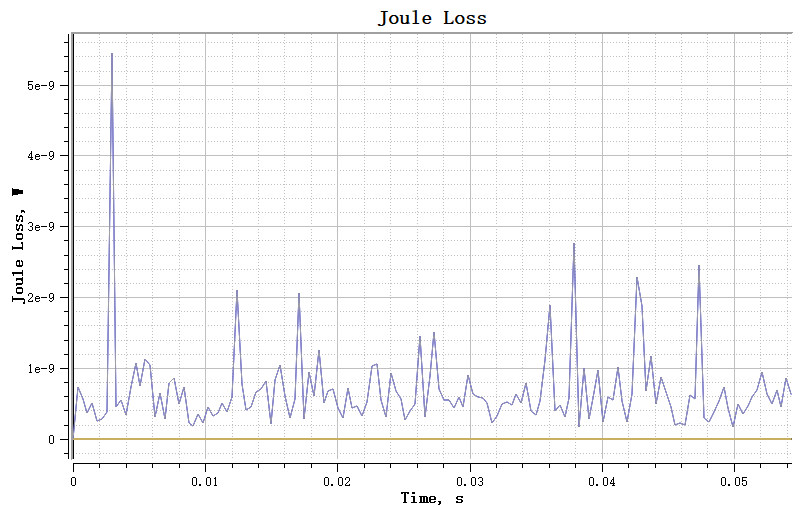
\includegraphics[width=1\linewidth]{./img/task3/joule-n4.png}
  \caption{空载条件下的磁滞损耗,$n=4$}
\end{figure}
\begin{figure}[H]
  \centering
  \includegraphics[width=1\linewidth]{./img/task3/joule-n8.png}
  \caption{空载条件下的磁滞损耗,$n=8$}
\end{figure}
\begin{figure}[H]
  \centering
  \includegraphics[width=1\linewidth]{./img/task3/joule-n10.png}
  \caption{空载条件下的磁滞损耗,$n=10$}
\end{figure}

\subsection{负载性能对比}

用电流源模拟负载,电流源模型参数如下:
\begin{figure}[H]
  \centering
  \includegraphics[width=0.8\linewidth]{./img/task2/load.png}
  \caption{负载条件下的电路图}
\end{figure}
\begin{figure}[H]
  \centering
  \includegraphics[width=0.8\linewidth]{./img/task2/load-config.png}
  \caption{电流源参数配置(峰值10A)}
\end{figure}

\subsubsection{电压}
负载条件下的电压表现取决于电机的设计和负载特性。
\begin{itemize}
	\item 4极电机:在高速运行下,可能会表现出较大的电压降。这是因为在高速运行时,电机的内阻和感抗会对电压产生更大的影响。
	\item 8极和10极电机:由于运行速度较低,电压降可能较小。低速运行时,电机的内阻和感抗对电压的影响相对较小,因此在负载条件下,电压表现可能更加稳定。
\end{itemize}

\begin{figure}[H]
  \centering
  \includegraphics[width=1\linewidth]{./img/task3/voltage-n4-load.png}
  \caption{负载条件下的电压波形,$n=4$}
\end{figure}
\begin{figure}[H]
  \centering
  \includegraphics[width=1\linewidth]{./img/task3/voltage-n8-load.png}
  \caption{负载条件下的电压波形,$n=8$}
\end{figure}
\begin{figure}[H]
  \centering
  \includegraphics[width=1\linewidth]{./img/task3/voltage-n10-load.png}
  \caption{负载条件下的电压波形,$n=10$}
\end{figure}

\subsubsection{反电势}
\begin{itemize}
	\item 4极电机:由于磁场分布相对较不均匀,其反电势的谐波成分通常较高,这可能导致更多的电磁干扰和效率损失。
	\item 8极和10极电机:更高的极数有助于实现更均匀的磁场分布,因此它们的反电势谐波成分通常较低,这有利于提高电机的效率和降低电磁干扰。
\end{itemize}

\begin{figure}[H]
  \centering
  \includegraphics[width=1\linewidth]{./img/task3/FEM-n4-load.png}
  \caption{负载条件下的反电势波形,$n=4$}
\end{figure}
\begin{figure}[H]
  \centering
  \includegraphics[width=1\linewidth]{./img/task3/FEM-n8-load.png}
  \caption{负载条件下的反电势波形,$n=8$}
\end{figure}
\begin{figure}[H]
  \centering
  \includegraphics[width=1\linewidth]{./img/task3/FEM-n10-load.png}
  \caption{负载条件下的反电势波形,$n=10$}
\end{figure}

\subsubsection{转矩}
\begin{itemize}
	\item 4极电机:当负载增加时,4极电机能够提供较高的转矩,适用于需要快速响应和较大动力的应用。在负载条件下,转矩脉动可能较大,这可能导致机械振动和噪音。
	\item 8极和10极电机:这些电机在负载条件下提供的转矩虽然较低,但转矩输出更加平滑和均匀。这使得它们适合于精密控制和稳定性要求较高的应用,如精密制造和某些类型的机器人技术。
\end{itemize}

\begin{figure}[H]
  \centering
  \includegraphics[width=1\linewidth]{./img/task3/torque-n4-load.png}
  \caption{负载条件下的转矩,$n=4$}
\end{figure}
\begin{figure}[H]
  \centering
  \includegraphics[width=1\linewidth]{./img/task3/torque-n8-load.png}
  \caption{负载条件下的转矩,$n=8$}
\end{figure}
\begin{figure}[H]
  \centering
  \includegraphics[width=1\linewidth]{./img/task3/torque-n10-load.png}
  \caption{负载条件下的转矩,$n=10$}
\end{figure}

\subsubsection{电力输出}
一般来讲,电力输出的影响因素有以下两个方面:

转速:电机的转速直接影响其电力输出。通常,转速越高,电机的电力输出也越大。

转矩:转矩是另一个决定电力输出的重要因素。在给定的转速下,转矩越大,电力输出也越大。

对比图像可以发现,电力输出8极最大,10极次之。

对于4极电机而言,由于转速高,4极电机通常能提供较高的电力输出,特别是在需要高速运行的应用中。

对于8极和10极电机而言,由于转速较低,这些电机的电力输出通常低于4极电机。
但考虑转矩的影响,因此8极成为了在现有条件下电力输出最大的模型。
并且由于转矩分布更均匀,它们在提供持续稳定功率方面更为有效。
\begin{itemize}
	\item 
	\item 
\end{itemize}

\begin{figure}[H]
  \centering
  \includegraphics[width=1\linewidth]{./img/task3/power-n4-load.png}
  \caption{负载条件下的电力输出,$n=4$}
\end{figure}
\begin{figure}[H]
  \centering
  \includegraphics[width=1\linewidth]{./img/task3/power-n8-load.png}
  \caption{负载条件下的电力输出,$n=8$}
\end{figure}
\begin{figure}[H]
  \centering
  \includegraphics[width=1\linewidth]{./img/task3/power-n10-load.png}
  \caption{负载条件下的电力输出,$n=10$}
\end{figure}

\subsection{极对数对比小结}
在综合评估电机极数对其性能的影响时,我们发现4极、8极和10极电机各有其独特的特点和适用场景。4极电机通常在空载反电势和谐波方面表现出较高的值,这可能会导致效率损失和电磁干扰,但同时它们能够提供较高的峰值转矩,尽管伴随着较大的转矩脉动。这种类型的电机适合于需要快速响应和高动力输出的应用,比如某些工业和运输设备。然而,这些电机在高速运行时的磁滞损耗可能较高,且可能出现较大的电压降,这些因素需要在设计时考虑以优化其性能。

相比之下,8极和10极电机通常在低速应用中表现更佳,提供较低的空载反电势和谐波含量,有利于提高效率和减少电磁干扰。这些电机的转矩输出虽然在峰值上低于4极电机,但更加平滑和均匀,适合于需要精确控制和稳定性的应用,如精密制造和某些类型的机器人技术。在这些电机中,磁滞损耗和电压降通常更低,有助于提高整体效率和稳定性。

最后,考虑到电力输出,4极电机在高速应用中通常能提供较高的电力输出,而8极和10极电机则更适合于低速、高扭矩的应用场景。因此,在选择电机时,不仅要考虑极数,还需要综合考虑转速、转矩、效率、噪音水平以及特定应用的要求。每种极数的电机都有其优势和局限,正确的选择将基于对特定应用需求的深入理解。

\section*{写在最后}
在完成基于JMAG软件的三相永磁同步电机仿真分析的实验过程中,我经历了一段丰富而深刻的学习旅程,
对此我十分高兴并满怀感激之情。

首先,我要感谢我们的指导老师,您对三相永磁同步电机领域的深入讲解和专业指导,
使我得以将课堂上的理论知识与JMAG软件的实际操作相结合,从而深化了我的理解和掌握。
每次课堂上的精彩讲解都是如同指引航标,引导我在控制理论的海洋中航行。
这次实验不仅仅是对我所学知识的应用,更是一次宝贵的实践机会,
让我对永磁同步电机的工作原理有了更加深刻的认识。

同时,我也要特别感谢那些在网络上分享知识和经验的前辈和同行。
他们的文章和讨论为我提供了宝贵的参考资料,帮助我在遇到困难时找到了解决问题的思路。
特别是那些详细的JMAG操作指南\cite{IDAJ}\cite{JMAG-C2}\cite{JMAG-C3}和案例分析\cite{JMAG-Course},让我在学习JMAG软件使用过程中少走了许多弯路,对此我深表感激。

我也要特别感谢方桂安学长。虽然去年的作业要求与今年的不同,
但学长去年在博客上分享的报告\cite{JMAG}对我产生了深远的影响。在他的报告中,
我看到了深入浅出的解析和清晰的逻辑思维。您的报告让我深受启发,
也使我对电机的学习有了更深的认识和理解。我把您的博客网址和引用都标在了文末,
以表达我对您贡献的尊重和感谢。

这个实验过程不仅仅是对专业知识的应用,更是一次自我挑战和成长的历程。
在实验中,我不断地查阅资料,深入研究,理解和吸收了很多课堂上没有完全明白的知识点。
每一个小的发现和进步都让我感到无比的兴奋和满足。
然而,我也意识到我的水平还相当有限,还有很多东西我完全不了解或是一知半解,还有很多知识等待我去探索和学习。
我将把握住这次作业的契机,继续深入学习电机相关知识,争取能够了解很多,学会更多。

本着开源精神,我也将本次作业的所有模型和完成报告所用的\LaTeX 源文件全部托管在了GitHub仓库中,
以便老师和同学们进行浏览。

我诚挚地邀请每一位对此感兴趣的老师和同学,前往我的GitHub仓库查阅代码,
提出您的宝贵建议和批评。任何形式的反馈和建议,无论是关于代码的优化,
还是对于实验方法和结果的讨论,我都将热烈欢迎。我将珍惜所获得的一切知识和经验,
并继续在电机学的学习道路上不懈努力.


GitHub repository URL: 

\href{https://github.com/pbcn2/2023-HW-JMAG-three\_phase\_PMSM}{https://github.com/pbcn2/2023-HW-JMAG-three\_phase\_PMSM}

%%%%%%%%%%%%%%%%%%%%%%%%%%%%%%%%%%%%%%%%%%%%%%%%%%%%%%%%%%%%%%%%
%  参考文献
%%%%%%%%%%%%%%%%%%%%%%%%%%%%%%%%%%%%%%%%%%%%%%%%%%%%%%%%%%%%%%%%
%  参考文献按GB/T 7714-2015《文后参考文献著录规则》的要求著录. 
%  参考文献在正文中的引用方法:\cite{bib文件条目的第一行}

\renewcommand\refname{\heiti\wuhao\centerline{参考文献}\global\def\refname{参考文献}}
\vskip 12pt

\let\OLDthebibliography\thebibliography
\renewcommand\thebibliography[1]{
  \OLDthebibliography{#1}
  \setlength{\parskip}{0pt}
  \setlength{\itemsep}{0pt plus 0.3ex}
}

{
\renewcommand{\baselinestretch}{0.9}
\liuhao
\bibliographystyle{gbt7714-numerical}
\bibliography{./TempExample}
}



\end{document}

